\documentclass[handout]{beamer}
\usepackage[utf8]{inputenc}
\usepackage{graphics}
\mode<presentation> {
\usetheme{unc}}
\setbeamertemplate{navigation symbols}{} % To remove the navigation symbols from the bottom of all slides uncomment this line

\usepackage{graphicx} % Allows including images
\usepackage{booktabs} % Allows the use of \toprule, \midrule and \bottomrule in tables


\usepackage{hyperref}
\hypersetup{linkcolor=blue,colorlinks=true}


% Remove symbols
\beamertemplatenavigationsymbolsempty


%\usetheme{default}

\usefonttheme{serif}

%----------------------------------------------------------------------------------------
%	TITLE PAGE
%----------------------------------------------------------------------------------------


\title[Development and Foreign Aid]{\LARGE{Development, Foreign Aid, and the Resource Curse}}
\author[POLI 150]{Steven Saroka}
\institute{POLI 150}
\date{11 April 2024}


\begin{document}

\begin{frame}
\titlepage % Print the title page as the first slide
\end{frame}


%----------------------------------------------------------------------------------------
%	PRESENTATION SLIDES
%----------------------------------------------------------------------------------------

\begin{frame} 
	\frametitle{\LARGE{Announcements}}
	\begin{itemize}
		\Large{
			\item Exam 2 on the 18th. Covers all material AFTER exam 1. 15-20 multiple choice questions, open-note, open-book. Opens at 12:01 AM on the 18th and closes at 11:59 PM. 1 hour and 15 minutes time limit. Can be taken from anywhere; no requirement to be in the classroom.
			
		}
	\end{itemize}
\end{frame}

\begin{frame} 
	\frametitle{\LARGE{Today's Class}}
	\begin{itemize}
		\Large{
			\item LDC definition
			\\~\\
			\item Causal factors of development
			\\~\\
			\item Political economy of development
			\\~\\
			\item Resource Characteristics 
			\\~\\ 
			\item The Resource Curse   
		}
	\end{itemize}
\end{frame}

\begin{frame} 
	\frametitle{\LARGE{Key Terms}}
	\begin{itemize}
		\item Less developed countries
		\item Import-substituting industrialization
		\item Export-oriented industrialization 
		\item Official development assistance
		\item Resources
		\item Resource curse
		\item Dutch disease
		\item Rentier state
		\item Petrodollar system
	\end{itemize}
\end{frame}

\begin{frame} 
\frametitle{\LARGE{Central Questions}}
\centering
\large{Why are some countries less developed than others, and what can be done to change that? Are countries that have access to rare, exportable natural resources worse off than countries that don't have access to such resources?}
\end{frame}


\begin{frame} 
\frametitle{\LARGE{Differences in Development}}
\begin{itemize}
	\large{
		\item \textbf{Less developed countries (LDCs)} are those states at a relatively low level of economic development. \pause
		\item As a policy goal, these states want to become more developed. \pause
		\item While the goal itself is uncontroversial, the steps necessary to develop can cause some conflicts of interest. \pause
		\item In particular, the paths to development often produce policy conflicts with \textbf{advanced, industrialized countries (AICs)}: those states at a high level of economic development.
	}
\end{itemize}
\end{frame}

%https://ourworldindata.org/grapher/human-development-index
\begin{frame} 
	\frametitle{\LARGE{HDI Across the World}}
	\begin{figure}[ht!]
		\centering
		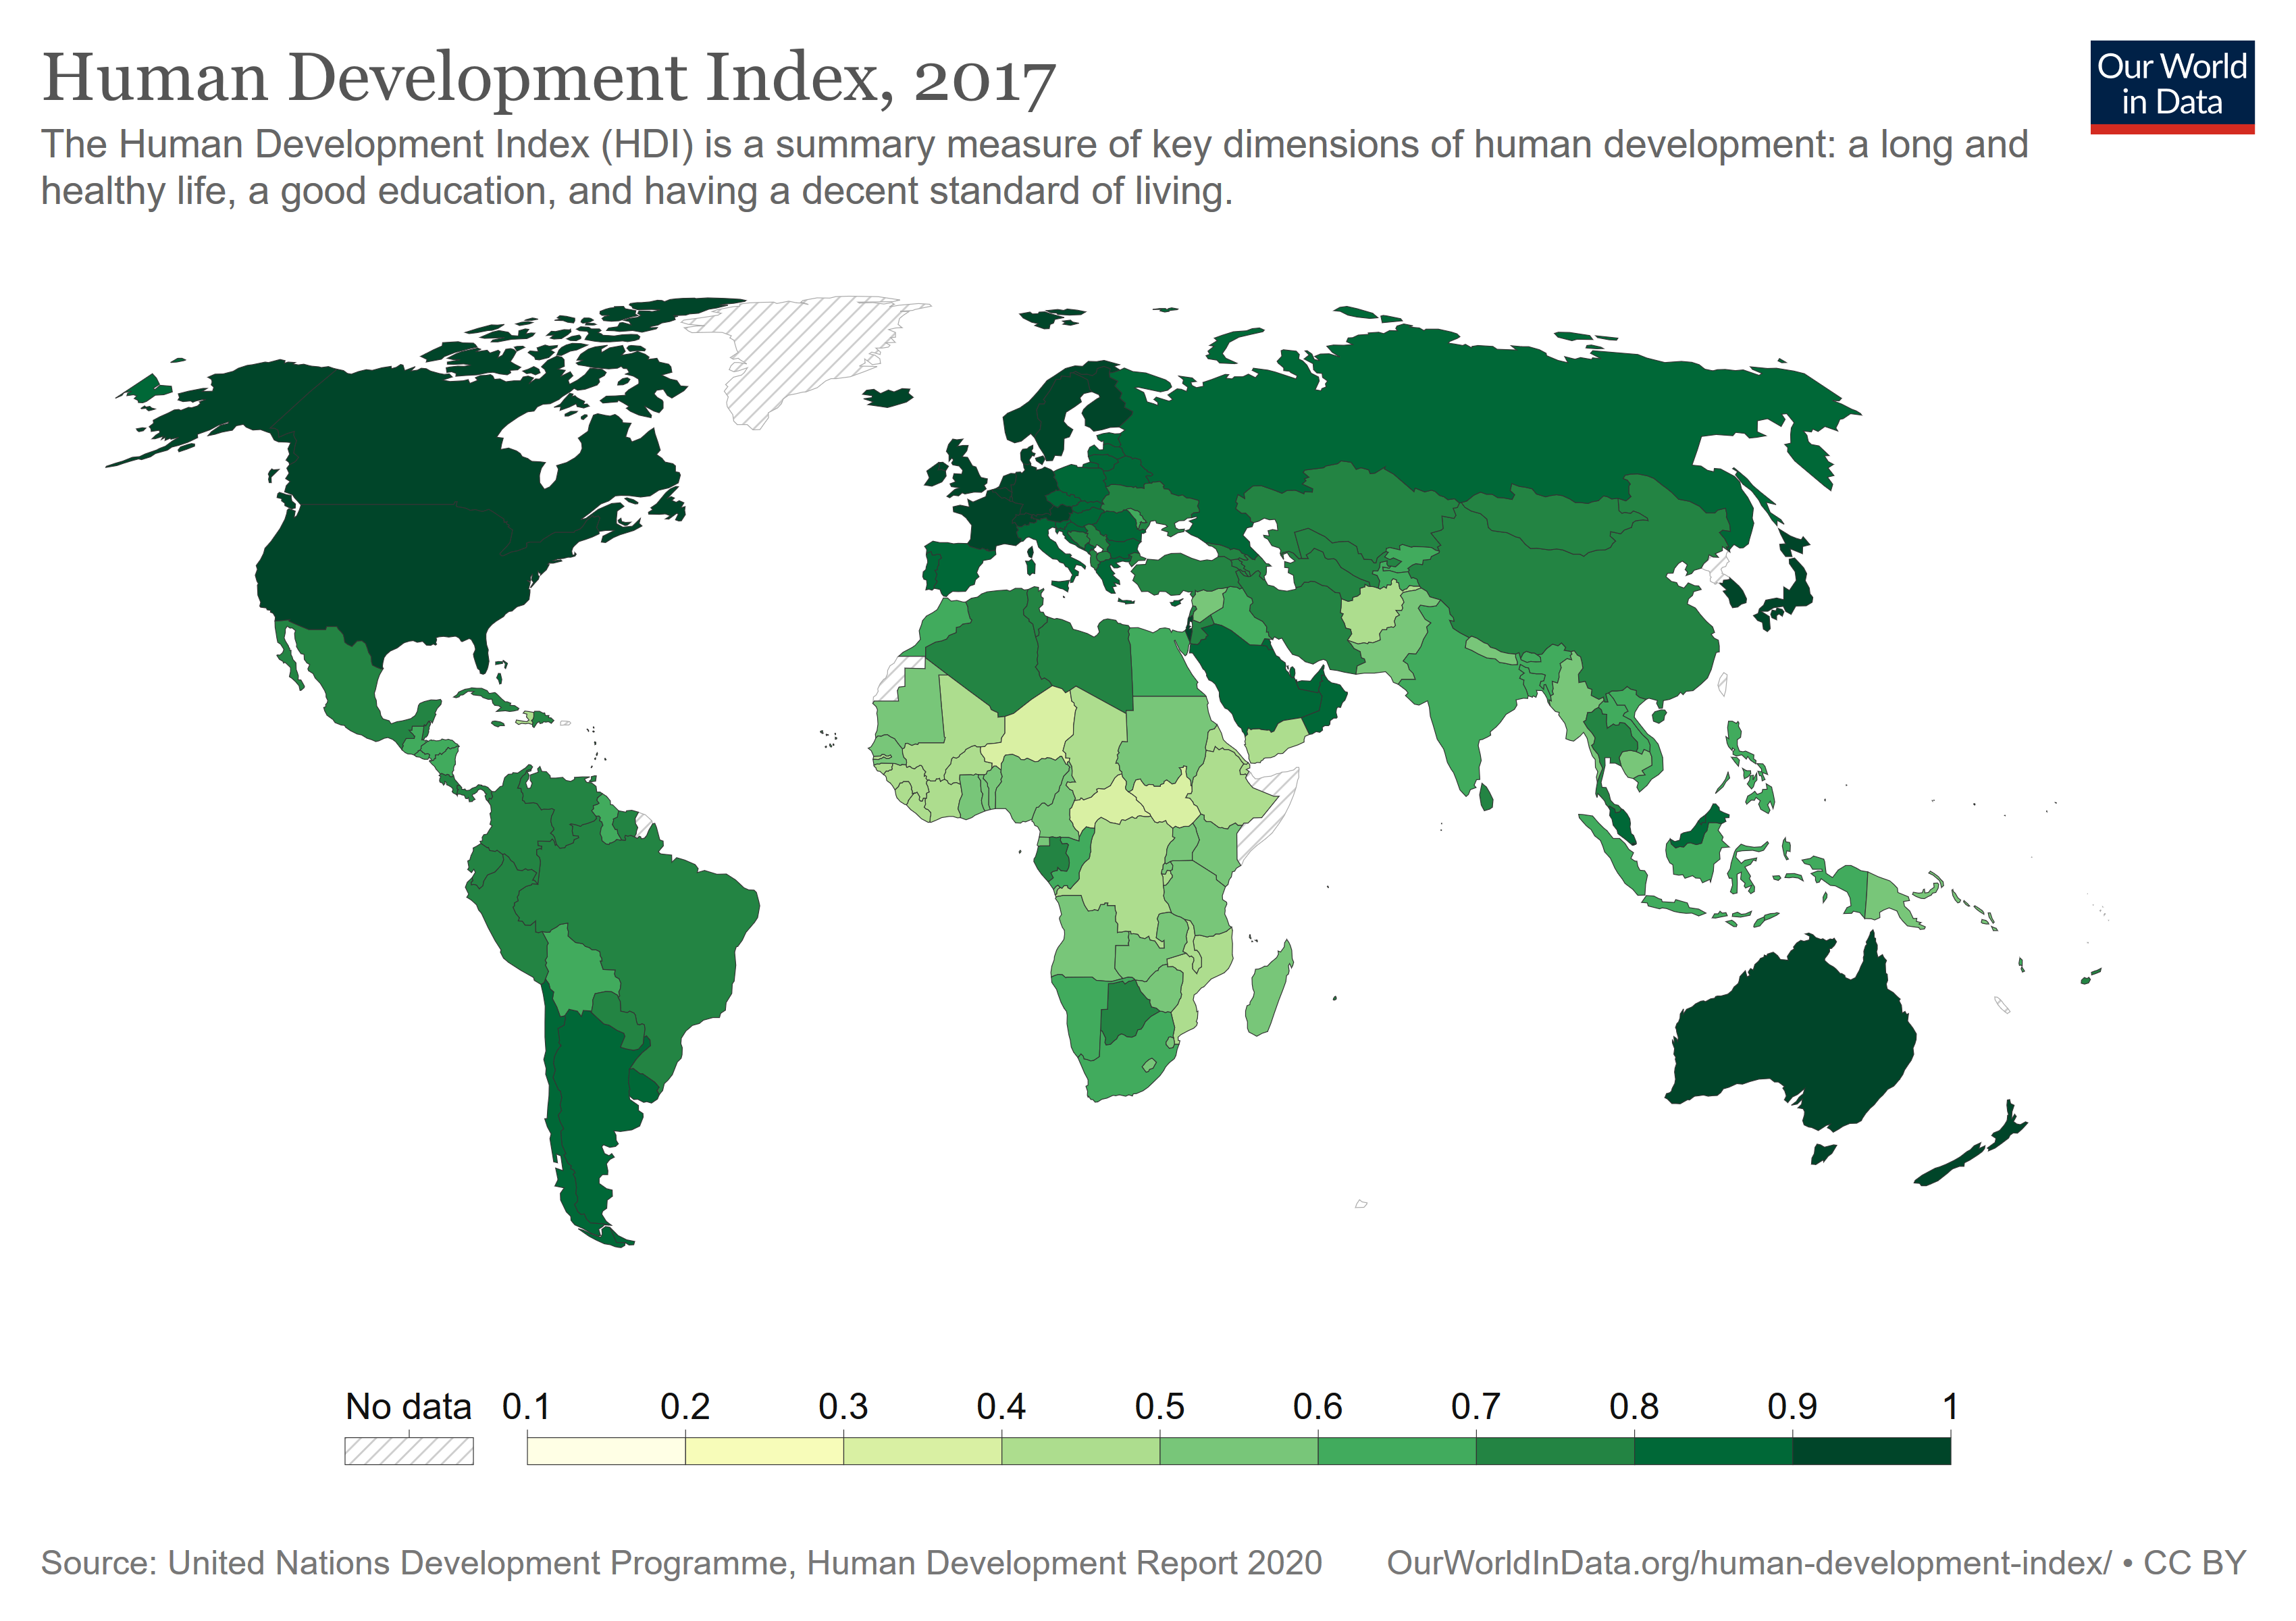
\includegraphics[height=\textheight, keepaspectratio]{./hdi.png}
	\end{figure}
\end{frame}

%https://ourworldindata.org/grapher/life-expectancy-vs-gdp-per-capita
\begin{frame} 
	\frametitle{\LARGE{GDPpc and Life Expectancy}}
	\begin{figure}[ht!]
		\centering
		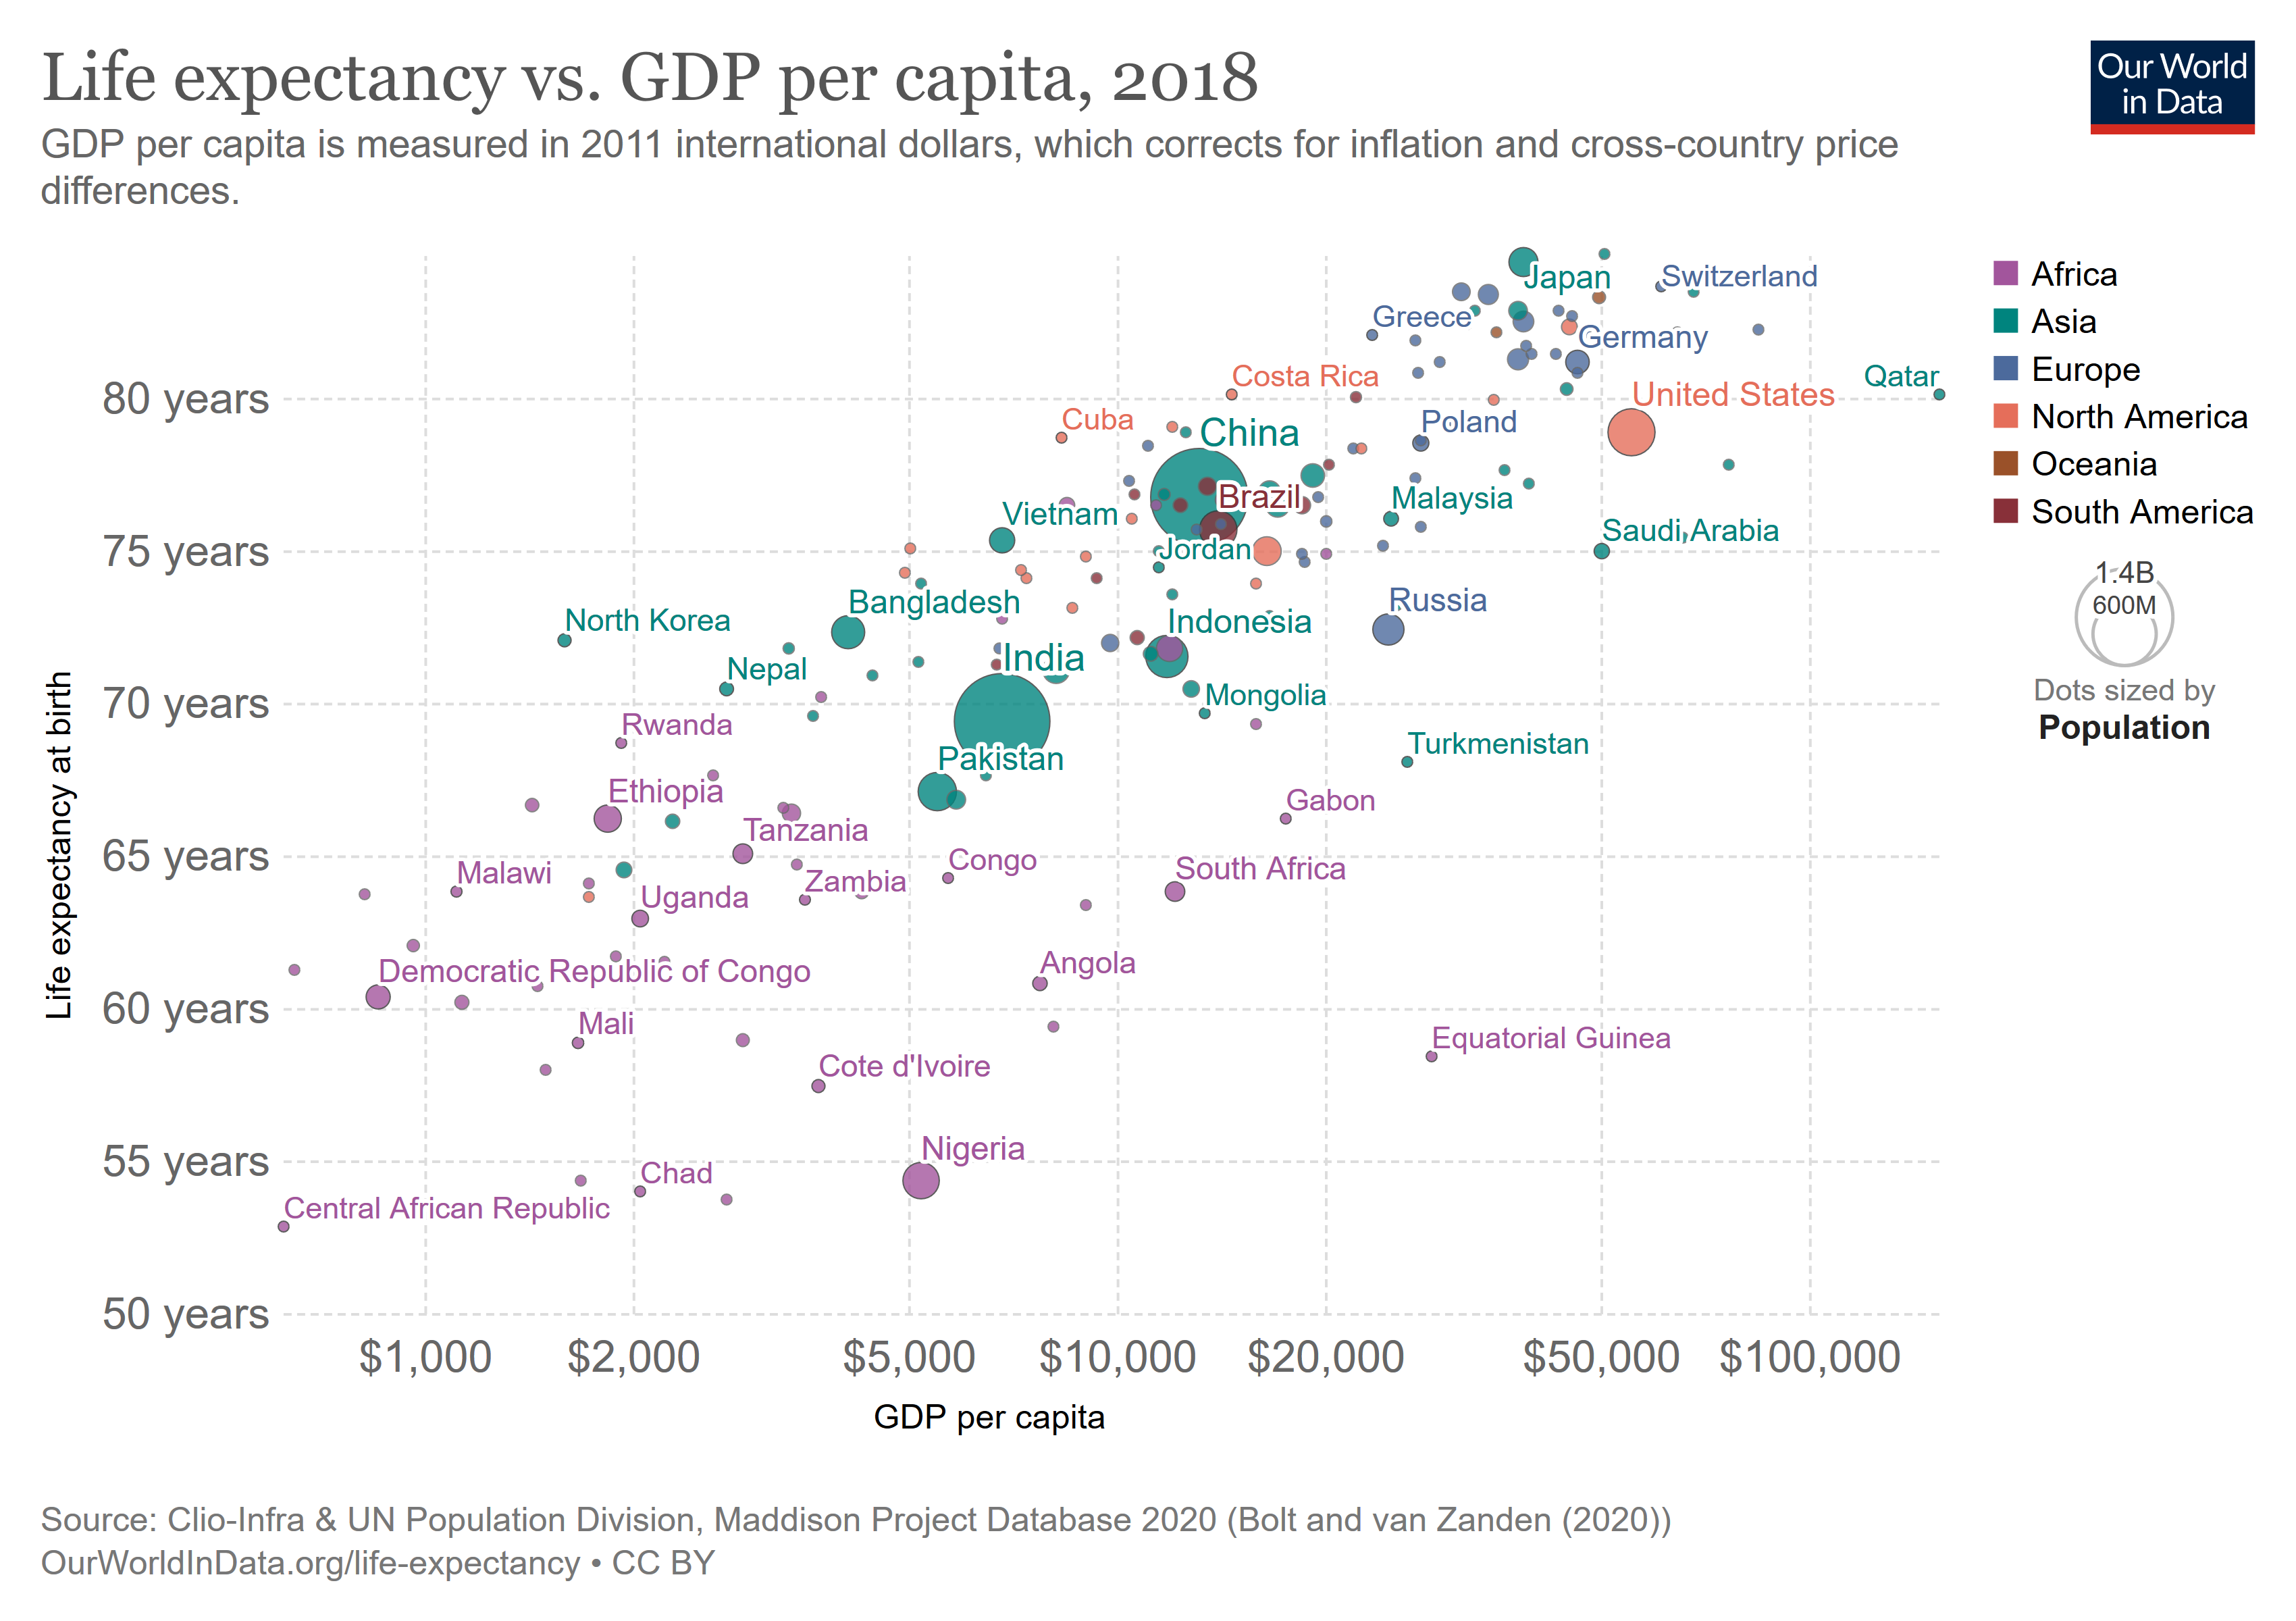
\includegraphics[height=\textheight, keepaspectratio]{life-expectancy-vs-gdp-per-capita.png}
	\end{figure}
\end{frame}

%https://ourworldindata.org/grapher/poverty-decline-without-china
\begin{frame} 
	\frametitle{\LARGE{Global Population and Poverty}}
	\begin{figure}[ht!]
		\centering
		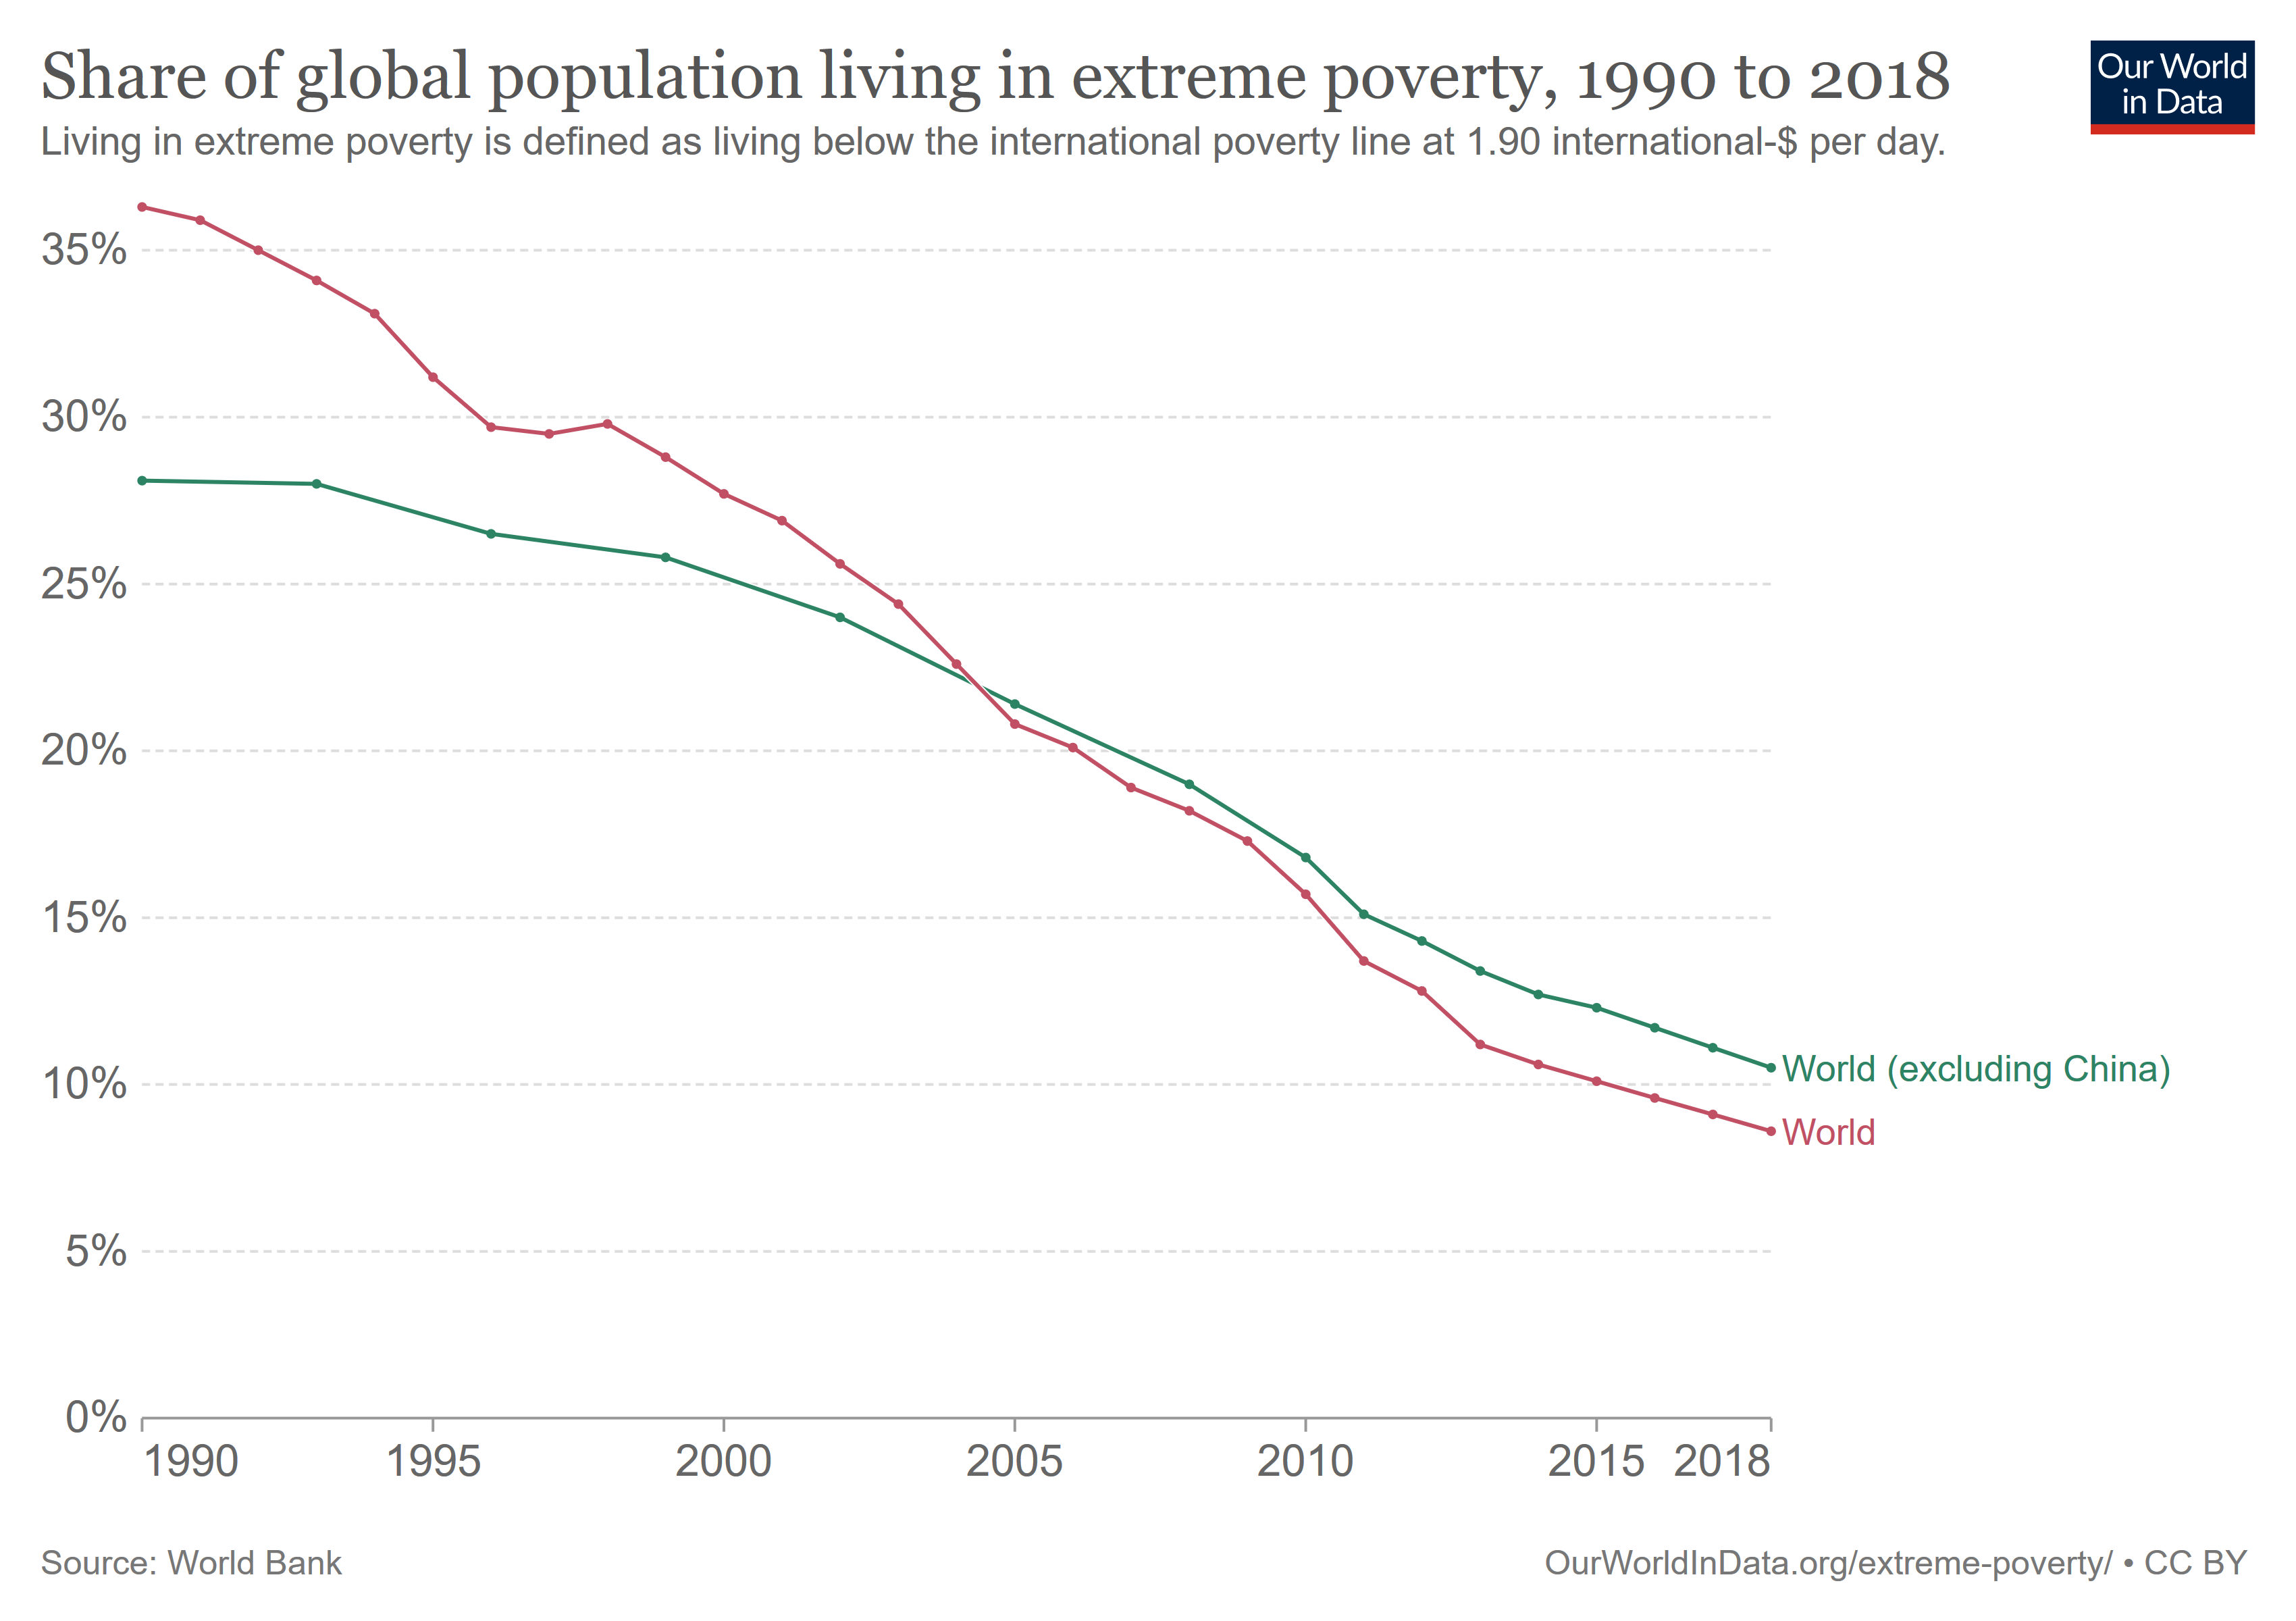
\includegraphics[height=\textheight, keepaspectratio]{poverty-decline-without-china.png}
	\end{figure}
\end{frame}

\begin{frame} 
	\frametitle{\LARGE{Poverty and GDPpc}}
	\begin{figure}[ht!]
		\centering
		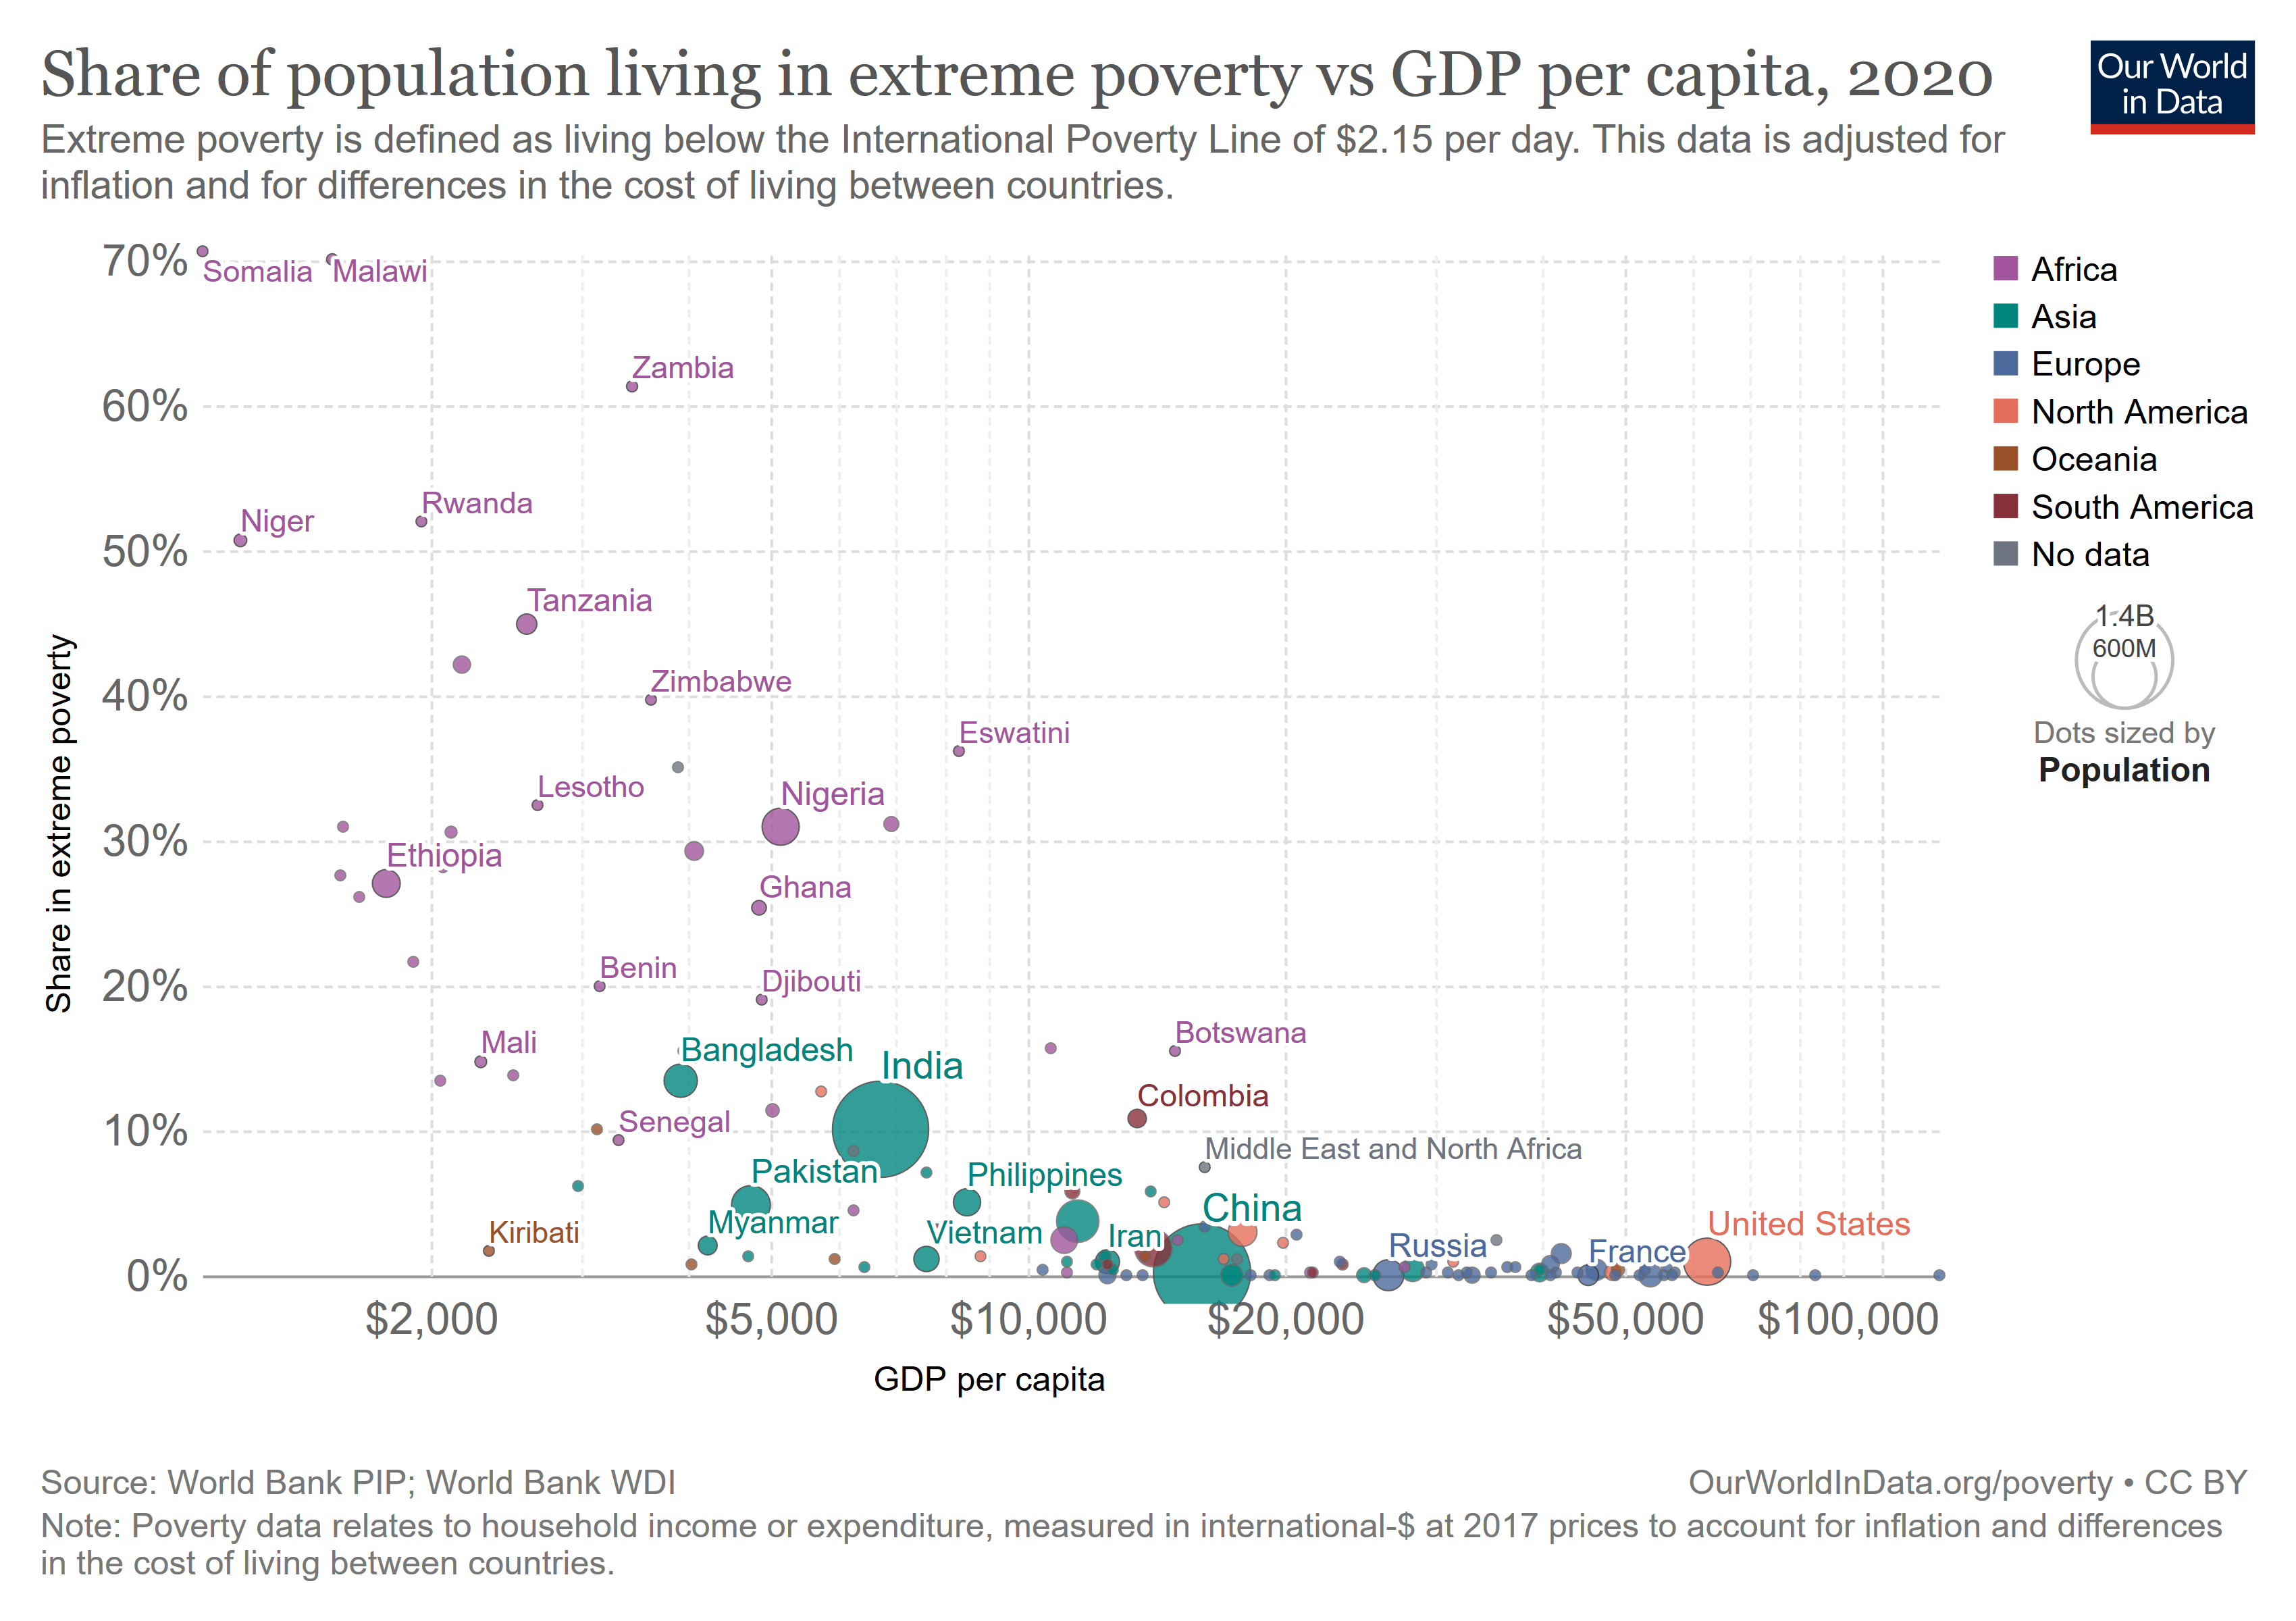
\includegraphics[height=\textheight, keepaspectratio]{poverty_vs_gdppc.png}
	\end{figure}
\end{frame}

\begin{frame} 
\frametitle{\LARGE{Stages of Development}}
\begin{itemize}
	\item The end goal of development efforts is uncontroversial: moving from a lower level of economic development to a higher level of economic development. \pause
	\item This shift means that the focus of economic activity shifts over time: 
	\begin{enumerate}
		\item Subsistence agriculture. \pause
		\item Primary sector: production of raw materials and farming. \pause
		\item Secondary sector: production of manufactured goods. \pause
		\item Tertiary sector: production of services. \pause
	\end{enumerate}
	\item Not the same sectors as in Ricardo-Viner theory!
\end{itemize}
\end{frame}

\begin{frame} 
	\frametitle{\LARGE{Stages of Development}}
	\begin{itemize}
		\item LDCs tend to focus on subsistence, primary sector production, and sometimes secondary sector production. \pause
		\item Advanced economies tend to focus the majority of their economic activity on the secondary and tertiary sectors. \pause
		\item These categories are abstractions and generalizations of the economy: you can find specific counter-examples for any of them.
		\item So, what aspects of a state explain its (lack of) development?
	\end{itemize}
\end{frame}

\begin{frame} 
\frametitle{\LARGE{Uncontrollable Aspects: Geography}}
\begin{itemize}
		\item Historians have long noticed that tropical regions are generally poor, while temperate regions are generally more wealthy. \pause
		\item Several potential explanations for this lack of development:
		\begin{itemize}
			\item Landlocked states \pause
			\item Distance from major markets \pause
			\item Diseases \pause
			\item Weather \pause
		\end{itemize}
		\item All of these were argued to lead to less development. 
\end{itemize}
\end{frame}

\begin{frame} 
	\frametitle{\LARGE{Uncontrollable Aspects: Geography}}
	\begin{itemize}
		\item Problem with this explanation: these geographical limitations were certainly true in the past, but less so in the modern era. \pause
		\item Bigger problem: Huge variation in countries that are geographically similar. \pause
		\item Ex: continued poverty in Zambia while Botswana has grown economically, despite similarly low levels of development at independence in the 1960s.
	\end{itemize}
\end{frame}


\begin{frame} 
\frametitle{\LARGE{Uncontrollable Factors: Colonialism}}
\begin{itemize}
		\item Colonialism is often cited as a source for lack of development. \pause
		\item The counterpoint is that many of the most developed countries in the world were colonies at one point. \pause
		\item But many policies of colonialism did hamper development: mercantilist trade toward mother country, restricted colonial manufacturing, resource exploitation. \pause
		\item To explain the difference in post-colonial experience, one must first examine the domestic determinants of growth.
\end{itemize}
\end{frame}

\begin{frame} 
\frametitle{\LARGE{Contestable Factors: Domestic Politics}}
\begin{itemize}
	\large{
		\item To promote growth, governments must provide: \pause
		\begin{itemize}
		    \item Infrastructure (roads, ports, etc.). \pause 
		    \item Secure property rights. \pause 
		    \item Stable economic policies.  
		\end{itemize}
	}
\end{itemize}
\end{frame}

\begin{frame} 
	\frametitle{\LARGE{Contestable Factors: Domestic Politics}}
	\begin{itemize}
		\large{
			\item Why do governments fail to do some of these things? \pause 
			\begin{itemize}
				\item Lack of technical capacity, resources. \pause 
				\item Lack of political will (e.g. conflict of interests between rural and urban areas). \pause
				\item Lack of strong government institutions able to do these things.
			\end{itemize}
			\item One explanation for differing colonial outcomes was that European colonists set up different institutions in different areas.
		}
	\end{itemize}
\end{frame}

\begin{frame} 
	\frametitle{\LARGE{Contestable Factors: Domestic Politics}}
	\begin{itemize}
		\item This argument, advanced by Acemoglu, Johnson, and Robinson (2001) and covered on pg. 440-441, says:
			\begin{itemize}
				\item European colonists only established growth-enabling government institutions with strong property rights protections, which ultimately encouraged investment, in areas where they could settle in large numbers without facing disease or other mortality factors. \pause
				\item In areas which were inhospitable to Europeans, they primarily set up extractive government institutions focused on siphoning wealth back to the motherland. These institutions, and this style of government, persisted after independence and sabotaged economic growth. \pause
			\end{itemize}
		\item \textbf{This account is largely discredited, based on methodological criticisms of the data analysis in that article, but the intuition has lingered.}
	\end{itemize}
\end{frame}

\begin{frame} 
	\frametitle{\LARGE{Development Policy}}
	\begin{itemize}
		\item In the modern era, and especially post-decolonization, the most obvious driver of economic growth was the development policy chosen by many LDCs. \pause
		\item This policy came in two types: ISI and EOI.
	\end{itemize}
\end{frame}


\begin{frame} 
	\frametitle{\LARGE{Policy Option: ISI}}
	\begin{itemize}
			\item \textbf{Import-substituting Industrialization (ISI)}: create protectionist barriers via high tariffs to close markets to imports, allowing local industry to develop free of foreign competition. \pause 
			\begin{itemize}
			    \item Practiced 1950s-1980s. \pause
			    \item Goal: industrialize via forcing the local production of formerly imported goods, which would eventually be competitive on the global market. \pause
			\end{itemize}
		\item Required substantial government involvement: trade barriers, government planning, investment policy choices.

	\end{itemize}
\end{frame}

\begin{frame} 
	\frametitle{\LARGE{Policy Option: ISI}}
	\begin{itemize}
		\item ISI was practiced from the 1950s-1980s. \pause
		\item ``Easy ISI" produced simple consumer goods.
		\item Secondary ISI focused on complex goods and machines as well as capital-intensive goods. \pause
		
	\end{itemize}
\end{frame}

\begin{frame} 
	\frametitle{\LARGE{Effects of ISI}}
	\begin{itemize}
		\item ISI produced economic growth in the 1960s and 1970s. \pause
		\item ISI led to general income redistribution from rural agriculture to urban manufacturing. \pause
		\item But failures and imbalances appeared in the 1970s... \pause
		\begin{itemize}
			\item Current account deficits and unsustainable sovereign borrowing eventually led to financial crises (starting with Mexico in 1982).
		\end{itemize}
		\item \textbf{More importantly, protected industries were not competitive once trade barriers were lowered.}
	\end{itemize}
\end{frame}


\begin{frame} 
	\frametitle{\LARGE{Policy Option: EOI}}
	\begin{itemize}
			\item Risks and failures of ISI led other developing states, especially those in East Asia, to look for a different approach. This led them to...
			\item \textbf{Export-Oriented Industrialization (EOI)}: support domestic manufacturing with loans, tax breaks, and currency management while remaining open to trade.  \pause 
			\item EOI was implemented during the 1980s, and (paradoxically) fit well with the Washington Consensus of the 1990s.
	\end{itemize}
\end{frame}

\begin{frame} 
	\frametitle{\LARGE{Policy Option: EOI}} 
		\begin{itemize}
			\item EOI produced sustainable growth for East Asian economies (Hong Kong, South Korea, Singapore, Taiwan). \pause
			\item Trade openness has benefited some developing countries significantly (China, India, Vietnam). \pause 
			\item Eventually became the major recommendation in IMF conditionality. 
		\end{itemize}

\end{frame}

\begin{frame} 
	\frametitle{\LARGE{EOI Caveats}} 
What are some potential shortcomings of the EOI model?
	\begin{itemize}
		\item Manufacturing competition is intense. \pause 
		\item First mover firms/states do well; later movers lose out. \pause 
		\item State must make accurate and effective long-term decisions regarding which sectors and industries it supports. \pause
		\item Harder to achieve productivity gains in non-manufacturing sectors, which is problematic in an information economy. \pause 
	\end{itemize}
Verdict: effective for those first East Asian states that adopted it, but less likely to succeed today.
\end{frame}

\begin{frame} 
	\frametitle{\LARGE{Biased Global Economy?}}
	As states have continued their development, some have raised concerns about the modern economy:
	\begin{itemize}
			\item AICs may have firmer control over their market prices, creating biased conditions in the global economy. \pause 
			\begin{itemize}
			    \item LDCs: produce primary products with many competitors. \pause 
			    \item AICs: produce specialized manufactured goods. \pause 
			\end{itemize}
			\item Moreover, AICs also protect their primary products, especially farmers, with trade barriers. \pause
			\begin{itemize}
			    \item Ex: in US 2020, farm subsidies were 48\% of farm income (\href{https://www.fb.org/market-intel/2022-farm-profitability-outlook-production-expenses-up-net-farm-income-down}{source}). \pause 
			    \item This lowers world prices, making it impossible for LDC farmers to compete.  
			\end{itemize}
	\end{itemize}
\end{frame}

\begin{frame} 
	\frametitle{\LARGE{Biased Global Economy?}}
	\begin{itemize}
		\item LDCs have had no success in convincing rich countries to lower agricultural barriers. \pause 
		\begin{itemize}
			\item IMF voting is a function of economy's size. \pause 
			\item WTO policy has lowered manufacturing trade barriers while allowing agriculture trade barriers to remain. \pause 
			\item LDCs formed the G77 (now 134) to advocate for LDC interests, but have not produced a new economic order.  
		\end{itemize}
	\end{itemize}
\end{frame}

\begin{frame} 
	\frametitle{\LARGE{AIC Policy Option: Foreign Aid}}
	\begin{itemize}
			\item One solution: share the wealth. \pause  
			\item \textbf{Official Development Assistance (ODA)/Foreign Aid}: Money or other assistance given to help countries developing economically or to meet basic needs. \pause 
			\begin{itemize}
			    \item Covers a variety of programs (political, economic, normative) \pause 
			    \item About 70\% is bilateral from AICs to LDCs \pause 
			    \item Relatively little foreign aid is directed at long-term economic development \pause 
			\end{itemize}
			\item AICs profess a goal of spending 0.7\% of GNI on foreign aid, but few do (and there is little political pressure to spend more).
	\end{itemize}
\end{frame}

%https://www.oecd.org/dac/financing-sustainable-development/development-finance-standards/official-development-assistance.htm
\begin{frame}{\LARGE ODA Expenditures 2020}
	\centering
	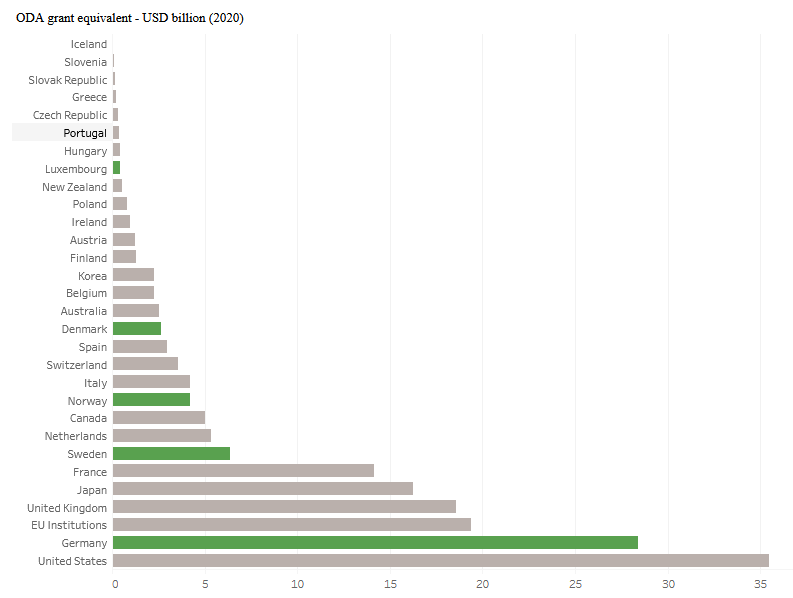
\includegraphics[width=\textwidth,height=.9\textheight,keepaspectratio]{ODAinUSD2020.png}
\end{frame}

%https://ourworldindata.org/grapher/net-oda-to-ldcs-as-percentage-of-donors-gni
\begin{frame}{\LARGE ODA Expenditures 2020}
    \centering
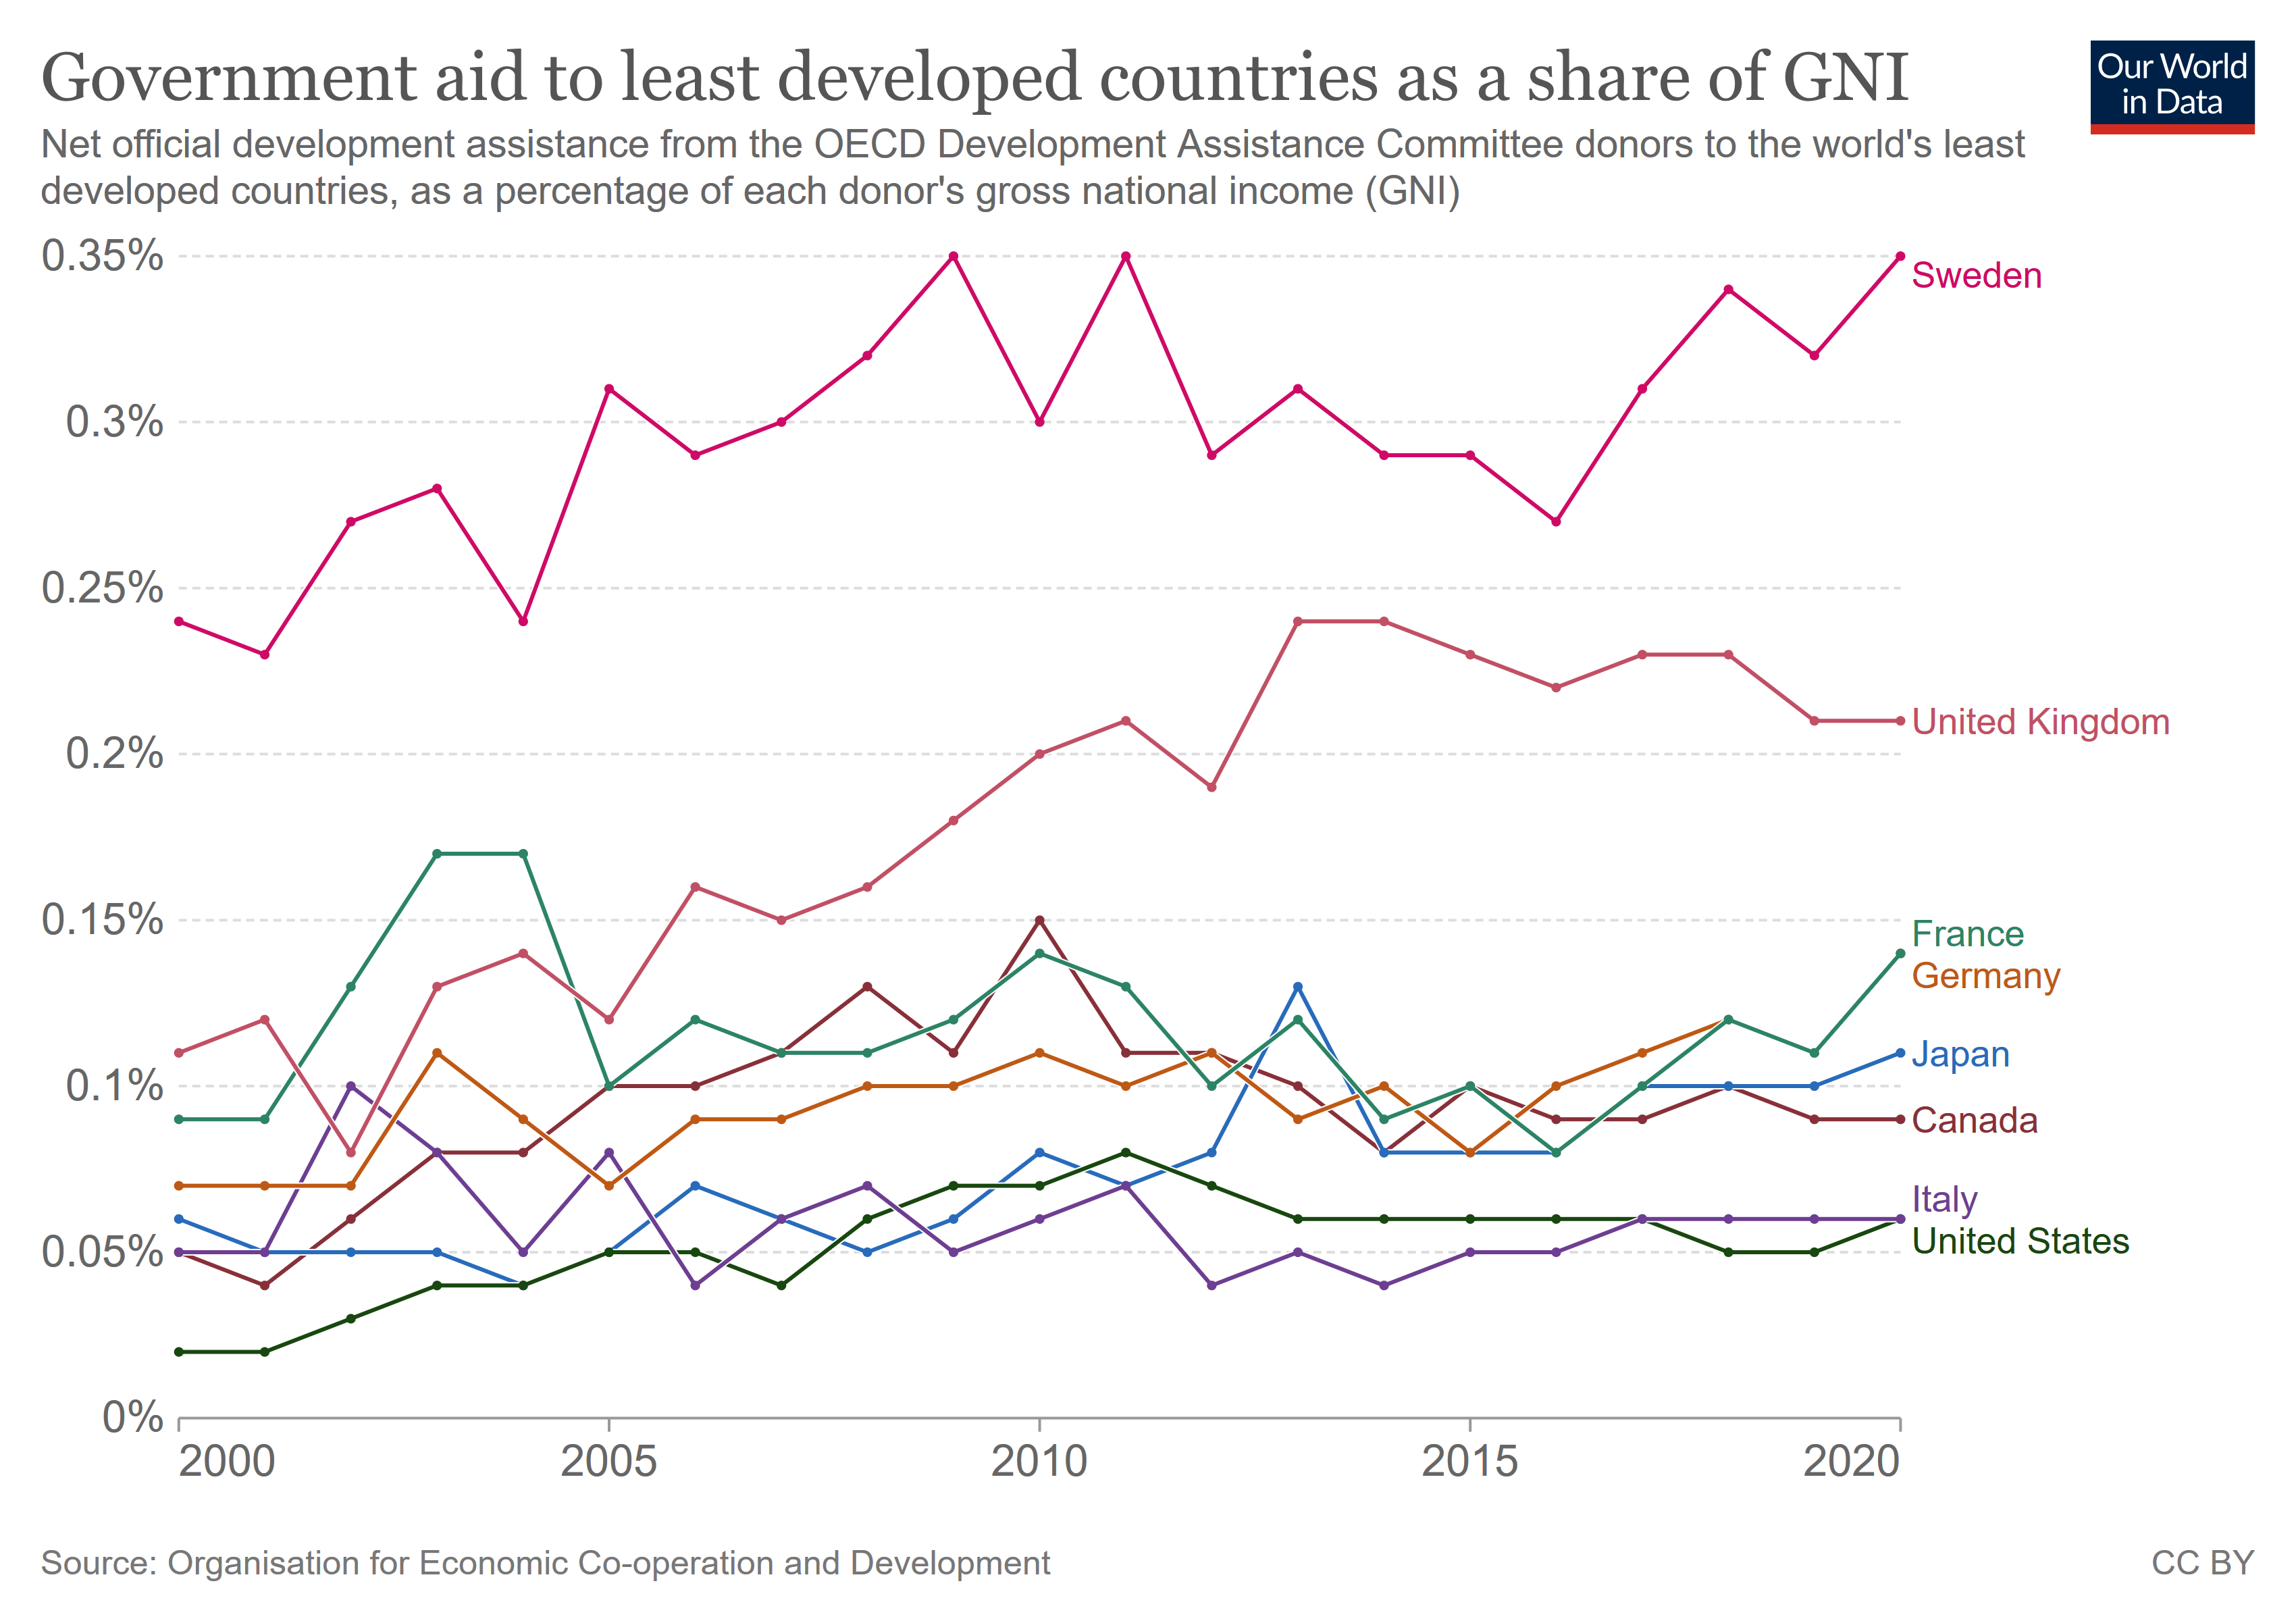
\includegraphics[width=\textwidth,height=.9\textheight,keepaspectratio]{ODAinGNI2020.png}
\end{frame}

\begin{frame} 
	\frametitle{\LARGE{US Foreign Aid vs. US Spending}}
	\begin{itemize}
		\item When surveyed, Americans report that they believe US foreign aid outflows are up to 20\% of government spending. \pause
		\item The reality is that US foreign aid is part of the international affairs budget of the federal government. \pause
		\item The overall international affairs budget (which includes diplomatic activities as well as aid ) is less than 1 percent of total federal spending.
	\end{itemize}
\end{frame}

\begin{frame}{\LARGE US Foreign Aid FY 2017}
	\centering
	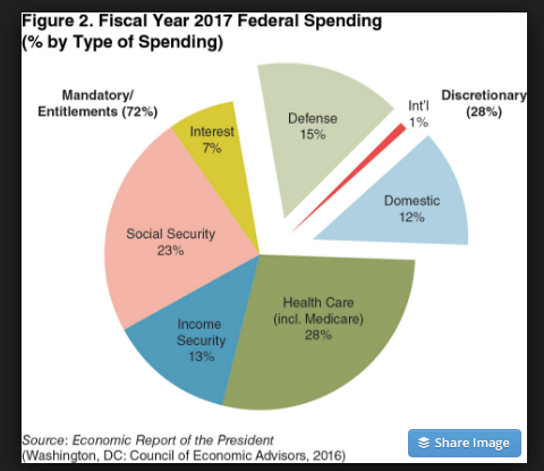
\includegraphics[width=\textwidth,height=\textheight,keepaspectratio]{USfedbudget.png}
\end{frame}

\begin{frame} 
	\frametitle{\LARGE{How is Aid Spent?}}
	\begin{itemize}
		\large{
			\item Aid can be motivated by strategic goals: \pause 
			\begin{itemize}
			    \item Alliances and post-conflict countries \pause 
			    \item Potential trade partners (create export markets) \pause 
			    \item Reduce emigration incentives \pause 
			\end{itemize}
			\item Some foreign aid is motivated by humanitarian and development goals: \pause 
			\begin{itemize}
			    \item UN's \href{https://www.un.org/sustainabledevelopment/sustainable-development-goals/}{Sustainable Development Goals} are at the heart of non-strategic aid. These are 17 goals intended to influence donor aid policies through 2030. \pause 
			\end{itemize}
		\item Substantial debate over whether and how aid is effective.
		}
	\end{itemize}
\end{frame}

\begin{frame} 
	\frametitle{\LARGE{Aid Effectiveness}}
Is aid effective at stimulating development? That is, is there a link between foreign aid and economic growth? \pause
	\begin{itemize}

		\item Prior research has not found consistent linkages at the country level. However, aid effects may be obscured by selection bias, as aid may be given for political or strategic reasons. \pause
		\item \href{https://www.aiddata.org/publications/aid-china-and-growth-evidence-from-a-new-global-development-finance-dataset}{Recent research} that statistically addresses selection effects finds an overall positive effect of US, total OECD-DAC and Chinese aid on growth.
	\end{itemize}
\end{frame}

\begin{frame} 
	\frametitle{\LARGE{Aid Effectiveness Continued}}
In addition to selection effects, aid may have unintended consequences...
	\begin{itemize}
		\item Aid may encourage corruption, and it can allow leaders to put off political reforms, as a kind of unearned income/rent. \pause
		\item At the subnational level, aid may not be allocated to the poorest areas within target states, but the richest areas (though this does not tell us whether the individuals in those areas are rich or poor) (\href{https://static1.squarespace.com/static/5acc1ee17e3c3a103525fb2b/t/5acd1cbe352f53f7b76961d2/1523391678922/Briggs+\%282017\%29+Aid+Target+Poorest.pdf}{Briggs 2017}).
		\item Different types of aid may also have different effects, further complicating the picture.
	\end{itemize}
\end{frame}

\begin{frame} 
	\frametitle{\LARGE{Summary: Conflicting Interests}}
	\begin{itemize}
		\item Both AICs and LDCs want to spur development globally (for economic, political, and humanitarian reasons). \pause 
		\begin{itemize}
			\item However, AICs are limited by what their domestic politics will accept (e.g. US and agriculture subsidies). \pause 
			\item ISI failed to help LDCs, and they cannot all gain equally from EOI (though EOI had some successes).  
		\end{itemize}
	\end{itemize}
\end{frame}

\begin{frame} 
	\frametitle{\LARGE{Summary: Conflicting Interests}}
	\begin{itemize}
		\item Sharing wealth (i.e. foreign aid) probably has some effect, but is not a cure-all: \pause 
		\begin{itemize}
			\item Easily derailed by strategic/political objectives \pause 
			\item Potential for resource curse (unearned income)\pause 
			\item Unclear what exactly is the most effective method \pause 
		\end{itemize}
		\item Thus, the competing visions between AICs and LDCs for what development looks like informs a great deal of economic conflict in IR. \pause 
		\begin{itemize}
			\item E.g. Doha Round of WTO collapsed in part due to agriculture. \pause 
			\item E.g. imbalance of power in tax agreements aimed at eliminating double taxation between rich states and LDCs.
		\end{itemize}
	\end{itemize}
\end{frame}

\begin{frame} 
	\frametitle{\LARGE{Resource Curse Intro}}
	\begin{itemize}
		\item Development may be complicated even more by a phenomenon called the \textbf{Resource Curse}.
		\item Defining this first requires defining what a ``resource" is...
		
	\end{itemize}
\end{frame}

\begin{frame} 
	\frametitle{\LARGE{Characteristics of Resources}}
	\begin{itemize}
		\large{  
			\item Naturally occurring, extractable resources (not produced). \pause 
			\begin{itemize}
				\item Generally minerals and fossil fuels: oil, diamonds, gold, cobalt, etc. \pause 
				\item Esp. materials used for fuel (including renewable energy). \pause 
			\end{itemize}
			\item Minimal labor required to extract them (compared to agriculture and manufacturing). \pause 
			\begin{itemize}
				\item Can be \textit{technologically} easy (alluvial diamonds) or difficult (oil). \pause 
			\end{itemize}
			
			\item Finite supply. \pause 
			
			\item Valuable as inputs into other processes. \pause 
			
			\item Highly portable, thus easily exported.
		}
	\end{itemize}
\end{frame}

\begin{frame} 
	\frametitle{\LARGE{Why Are These Resources Problematic?}}
	\begin{itemize}
		\large{
			\item Potential independent influence on political institutions. \pause
			
			\item Unlikely to enhance economic productivity in the long-term. \pause
			\begin{itemize}
				\item Low labor requirements, tech transfer unlikely, low incentives to increase productivity \pause
			\end{itemize}
			
			\item High value may inflate the currency and cost of business for other industries.  \pause
			
			\item Use as inputs means they're not necessarily directly useful to the economy. \pause
			
			\item Associated with environmental damage and climate change.
		}
	\end{itemize}
\end{frame}



\begin{frame} 
	\frametitle{\LARGE{Resource Curse Types}}
	\begin{itemize}
		\item Natural resources are empirically associated with three potential ``curses," creating \textbf{the resource curse}: \pause 
		\item \textbf{Economic}: \pause 
		\begin{itemize}
			\item Poor economic growth \pause 
			\item Poor long-term economic outcomes \pause 
		\end{itemize}
		\item \textbf{Political}:  \pause 
		\begin{itemize}
			\item Greater likelihood for civil conflict \pause 
			\item Worse governance and institutions  \pause 
		\end{itemize}
		\item \textbf{Social}:  \pause 
		\begin{itemize}
			\item Worse demographic and equality outcomes  \pause 
		\end{itemize}
		\item The resource curse seems to be particularly common in the developing world.
	\end{itemize}
\end{frame}





\begin{frame} 
	\frametitle{\LARGE{Resources and the Economy}}
	\begin{itemize}
		\large{
			\item Is resource wealth correlated with lower rates of economic growth?  \pause 
			\begin{itemize}
				\item Answers depend on the time frame of the analysis.  \pause 
			\end{itemize}
			\item Resource endowments are linked with greater growth \textbf{volatility}. \pause 
			\begin{itemize}
				\item 1974-1989: the more oil countries produced, the greater their economic decline. \pause 
				\item Resources often also linked with rising inequality. \pause 
			\end{itemize}
			\item By contrast, resource wealth was also linked with better child health. \pause 
			\begin{itemize}
				\item However, this linkage varies across regions: Middle East (strongest), Latin America, Africa (weakest).
			\end{itemize}
		}
	\end{itemize}
\end{frame}


%% Azerbaijan 
\begin{frame}{\LARGE Azerbaijan's Oil Boom}
	\centering
	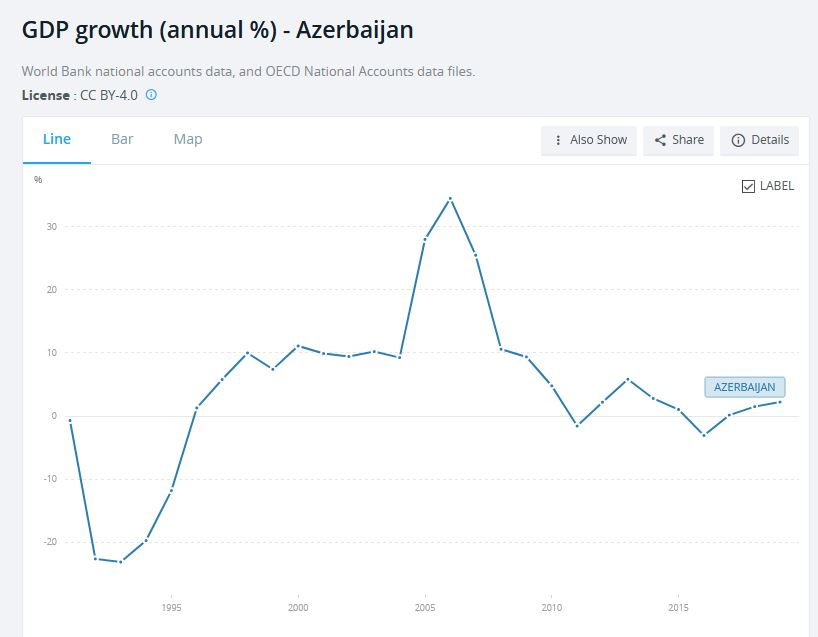
\includegraphics[width=\textwidth,height=0.8\textheight,keepaspectratio]{azerbaijan growth.JPG}
\end{frame}

% Azerbaijan inflation
\begin{frame}{\LARGE Inflation in Azerbaijan}
	\centering
	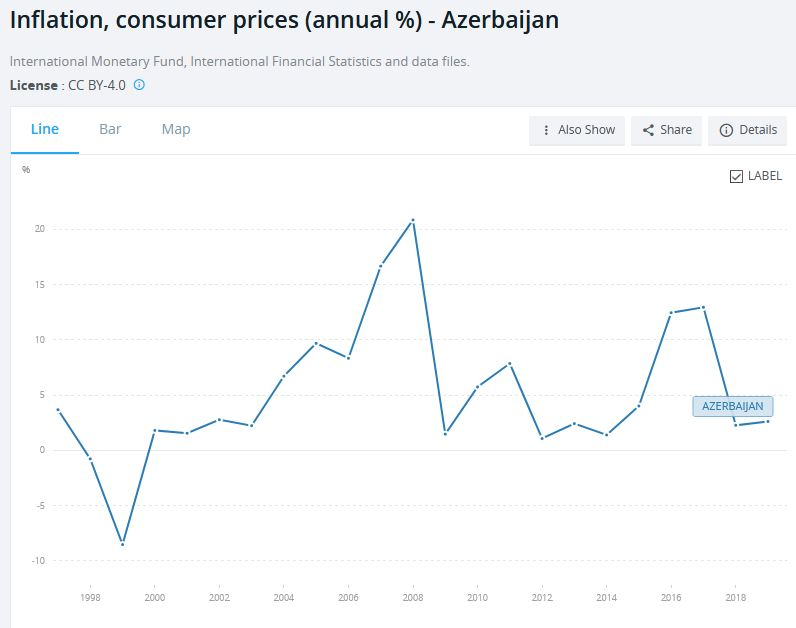
\includegraphics[width=\textwidth,height=0.8\textheight,keepaspectratio]{azerbaijan inflation.JPG}
\end{frame}


\begin{frame} 
	\frametitle{\LARGE{Resource Endowments and Growth}}
	\begin{itemize}
		\large{
			\item Ross (2015): resource-rich countries haven't grown any faster than any other countries. Why not? \pause 
			\item One explanation is \textbf{``Dutch disease"}: positive wealth shocks from the resource sector put upward pressure on prices throughout the economy. \pause 
			\item As labor and other input costs go up in the non-resource sectors, those firms become globally noncompetitive.  \pause 
			\item Wages in the resource sector deter workers and entrepreneurs from participation in other sectors, further weakening them.  \pause 
			\begin{itemize}
				\item Less innovation and skill acquisition in non-resource sectors.
			\end{itemize}
		}
	\end{itemize}
\end{frame}

%from Atlas of Economic Complexity; per Tyler: "Yep, that’s about it! It’s from something called the Atlas of Economic Complexity. The economists who made it created network of product spaces from trade data, with the point being that the more interconnected products are with each other, the more likely you are to see sustainable development, because you can have capital and labor move across industries"
%\begin{frame}{\LARGE Saudi Arabia's Product Space}
%	\centering
%	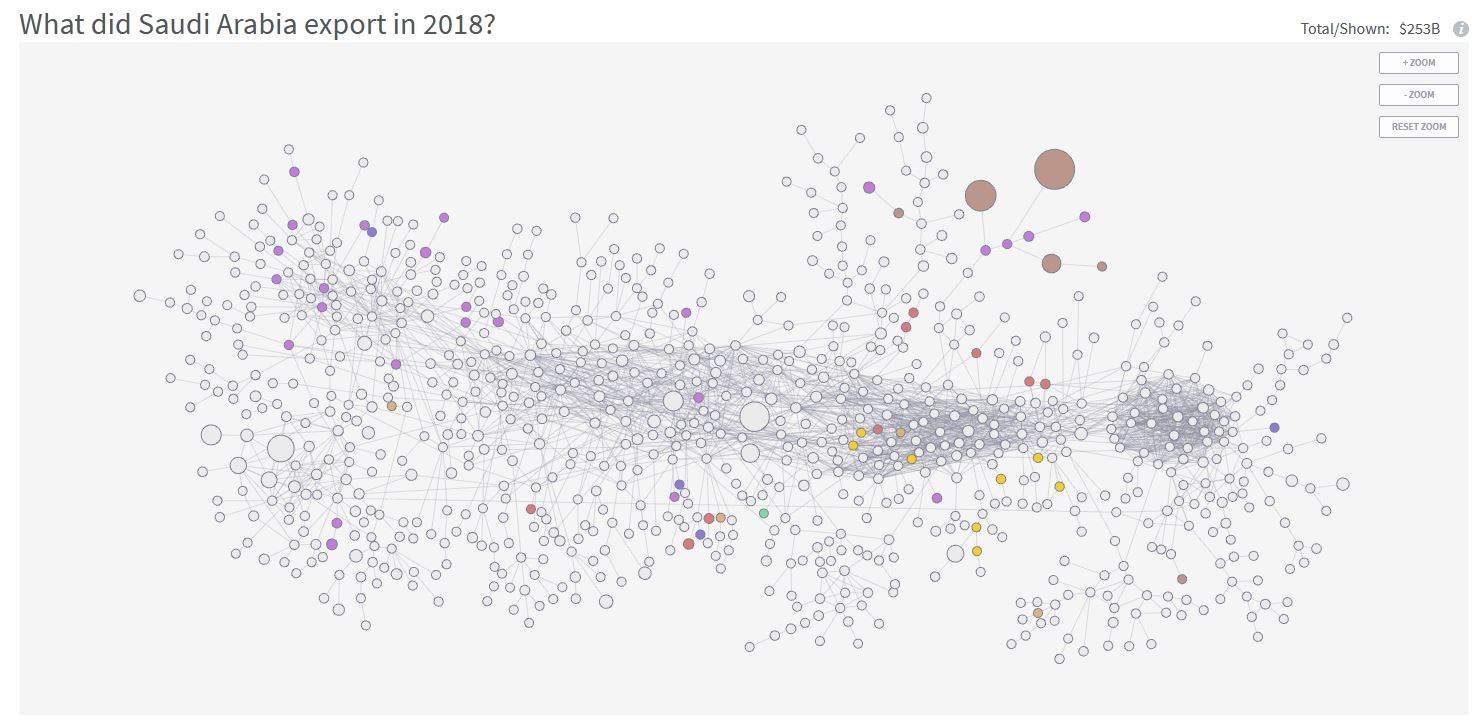
\includegraphics[width=\textwidth,height=0.8\textheight,keepaspectratio]{saudi arabia product space.JPG}
%\end{frame}


\begin{frame} 
	\frametitle{\LARGE{Resources and Civil Conflict}}
	\begin{itemize}
		\large{
			\item Positive and significant relationship between resources and the occurrence of civil war. \pause
			\begin{itemize}
				\item Effect present for both oil \textit{and} other natural resources. \pause
				\item Inverted U-shape relationship: at very high or low levels of resource wealth, probability of conflict lessens. \pause
				\item Example: Libyan civil war. \pause
			\end{itemize}
			\item Location of resource also matters: \pause
			\begin{itemize}
				\item Offshore vs. onshore oil wells. \pause
				\item More conflict in poor areas, and in areas dominated by ethnic minority. \pause
			\end{itemize}
			\item \textbf{No scholarly consensus on causal mechanisms behind this relationship, but it does exist.}
		}
	\end{itemize}
\end{frame}

%% Libya civil war
\begin{frame}{\LARGE Libya's Civil Conflict 2014-2020}
	\centering
	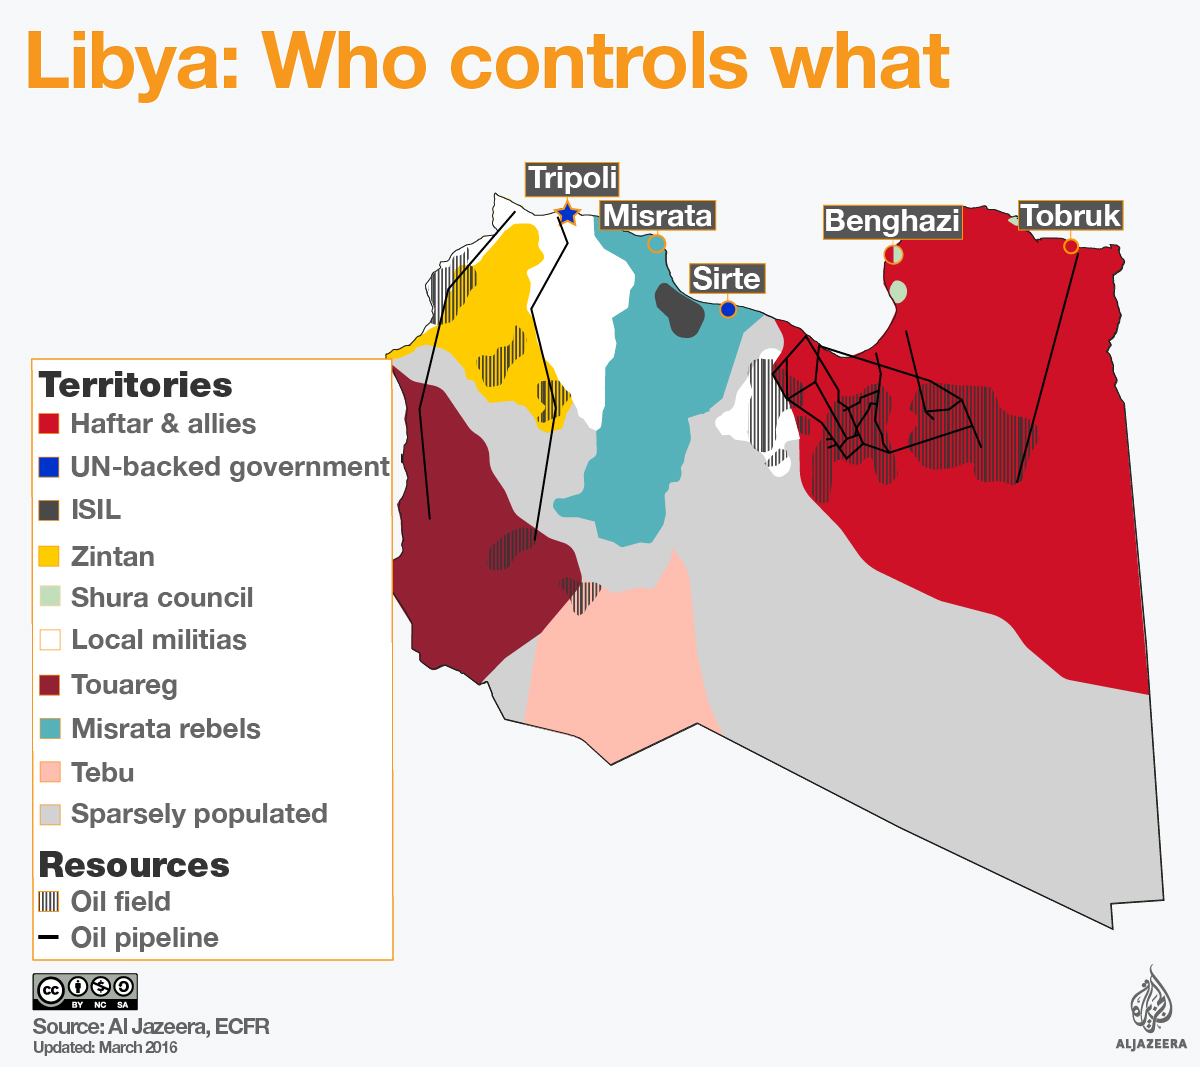
\includegraphics[width=\textwidth,height=0.8\textheight,keepaspectratio]{libya control.jpg}
\end{frame}

%% Sudan civil war
\begin{frame}{\LARGE Sudan's Civil Conflict (2013-2020)}
	\centering
	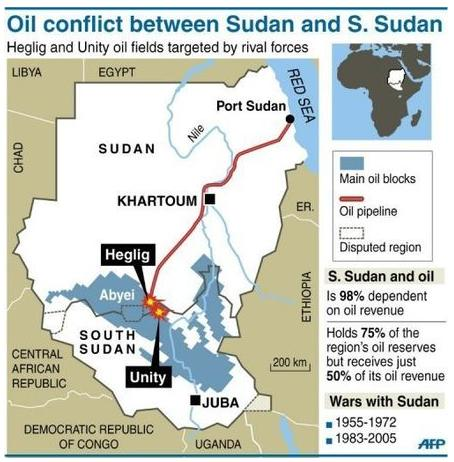
\includegraphics[width=\textwidth,height=0.8\textheight,keepaspectratio]{sudan oil fields.jpg}
\end{frame}




\begin{frame} 
	\frametitle{\LARGE{Resources and Domestic Institutions}}
	\begin{itemize}
		
		\item Higher levels of \textbf{oil} wealth help authoritarian regimes and rulers ward off democratic pressures. \pause
		\begin{itemize}
			\item Effect holds under certain conditions, such as nationalized oil industries. \pause
			\item Total level of resource wealth is more important than changes in it. \pause
		\end{itemize}
		\item The effect of resource wealth in democracies is less clear. \pause
		\begin{itemize}
			\item But it appears to bolster incumbents, meaning less leader turnover. \pause
		\end{itemize}
		\item How does this actually work? \pause
		\begin{itemize}
			\item \textbf{Unearned income} means fewer pressures for accountability if not dependent on taxation to fund government activities. \pause
		\end{itemize}
		\item This could also be the case for other types of ``unearned income" (e.g. foreign aid).
		
	\end{itemize}
\end{frame}

%% Regime type image from Ross
\begin{frame}{\LARGE Resources and Regime Type}
	\centering
	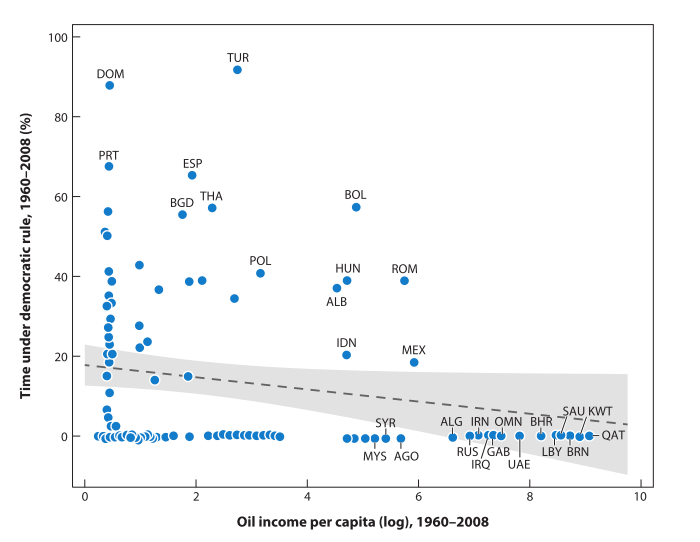
\includegraphics[width=\textwidth,height=0.8\textheight,keepaspectratio]{regime type.png}
\end{frame}

\begin{frame} 
	\frametitle{\LARGE{Resources and Society}}
	\begin{itemize}
		\large{
			\item There is a significant link between low levels of gender equality in politics and broader society, and resource wealth. \pause
			\begin{itemize}
				\item There also appears to be a link to low levels of income equality overall. \pause
			\end{itemize}
			\item Some resources appear to be linked to slave and child labor. \pause
			\item Resource wealth (particularly oil) generally connected with higher levels of corruption and lower bureaucratic efficacy. \pause
			\item Oil-rich countries are also less likely to be cooperative internationally. \pause
			\begin{itemize}
				\item E.g. most non-WTO members are resource-wealthy (Azerbaijan, Iran, Libya, South Sudan)
			\end{itemize}
		}
	\end{itemize}
\end{frame}

% Resource wealth social outcomes 
%\begin{frame}{\LARGE Resource Wealth and Positive Outcomes}
%    \centering
%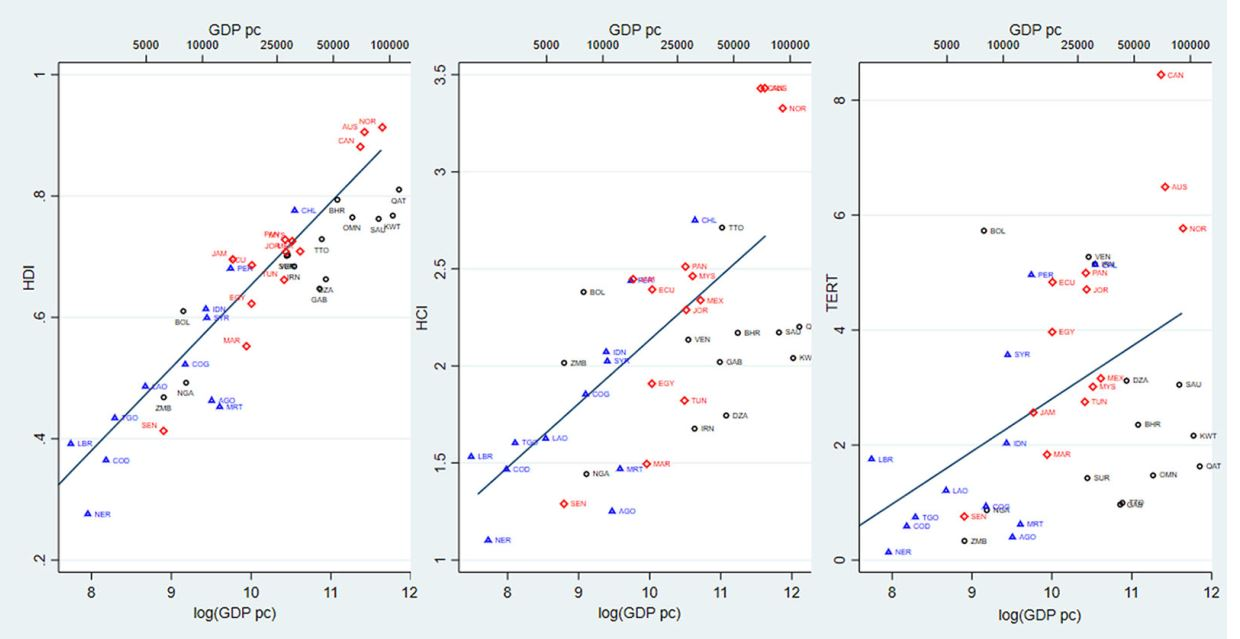
\includegraphics[width=\textwidth,height=0.8\textheight,keepaspectratio]{resource wealth social outcomes.JPG}
%\end{frame}


% Equality before the law
%\begin{frame}{\LARGE Equality Before the Law}
%	\centering
%	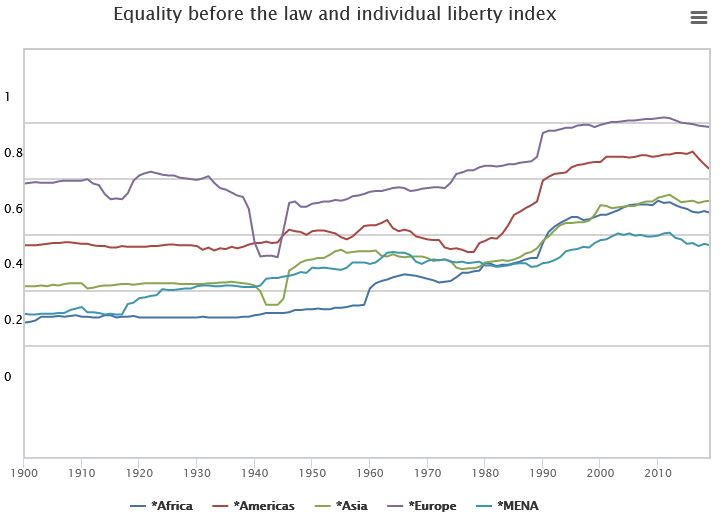
\includegraphics[width=\textwidth,height=0.8\textheight,keepaspectratio]{equality MENA.JPG}
%\end{frame}

\begin{frame} 
	\frametitle{\LARGE{Middle East and Oil}}
	\begin{itemize}
		\large{
			\item The Middle East is known for its concentration of oil wealth. \pause
			\begin{itemize}
				\item Revenue generated by oil exporters (Saudi Arabia, UAE, Iran) \pause
				\item Remittances (from employment in oil-rich economies) to the neighboring countries (Lebanon, Jordan, Egypt) \pause
				\item Most states possess oversized public sectors and function as \textbf{rentier states} that get a substantial portion of revenue from resource profits rather than taxation, and tend to be autocratic. \pause
				\item Thus, rentier states strike a bargain between state and citizens: low taxes and plentiful public sector jobs in return for lessened citizen input into government processes.
			\end{itemize}
		}
	\end{itemize}
\end{frame}

\begin{frame} 
	\frametitle{\LARGE{Middle East and Oil}}
	\begin{itemize}
		\large{
			\item The problem with the rentier state system is that it requires that profits continue to flow in, while the population remains at a stable level.
			\item As revenues decline and populations grow...\pause
			\begin{itemize}
				\item Fiscal pressure on governments increases \pause
				\item Some reforms in 2000s, but without accompanying political change\pause
				\item Some states trying to focus on improved education without new political accountability (ex: UAE)
			\end{itemize}
		}
	\end{itemize}
\end{frame}

\begin{frame} 
	\frametitle{\LARGE{Why is Oil Special?}}
	Much discussion of both resources and the resource curse is framed around oil. Why? \pause
	\begin{itemize}
		\large{  
			\item Widely distributed globally: variation both geographically and politically. \pause
			
			\item Energy input for manufacturing and transportation. \pause
			\begin{itemize}
				\item Necessary component of international trade and globalization. \pause
			\end{itemize}
			
			\item Strategic military asset. \pause 
			
			\item Relatively historically recent, thus vast untapped reserves. \pause 
			
			\item Technologically difficult to extract and to refine. \pause 
			
			\item Substantial negative effects on climate.
		}
	\end{itemize}
\end{frame}

%% Oil Distribution Chart
\begin{frame}{\LARGE Oil Distribution Globally}
	\centering
	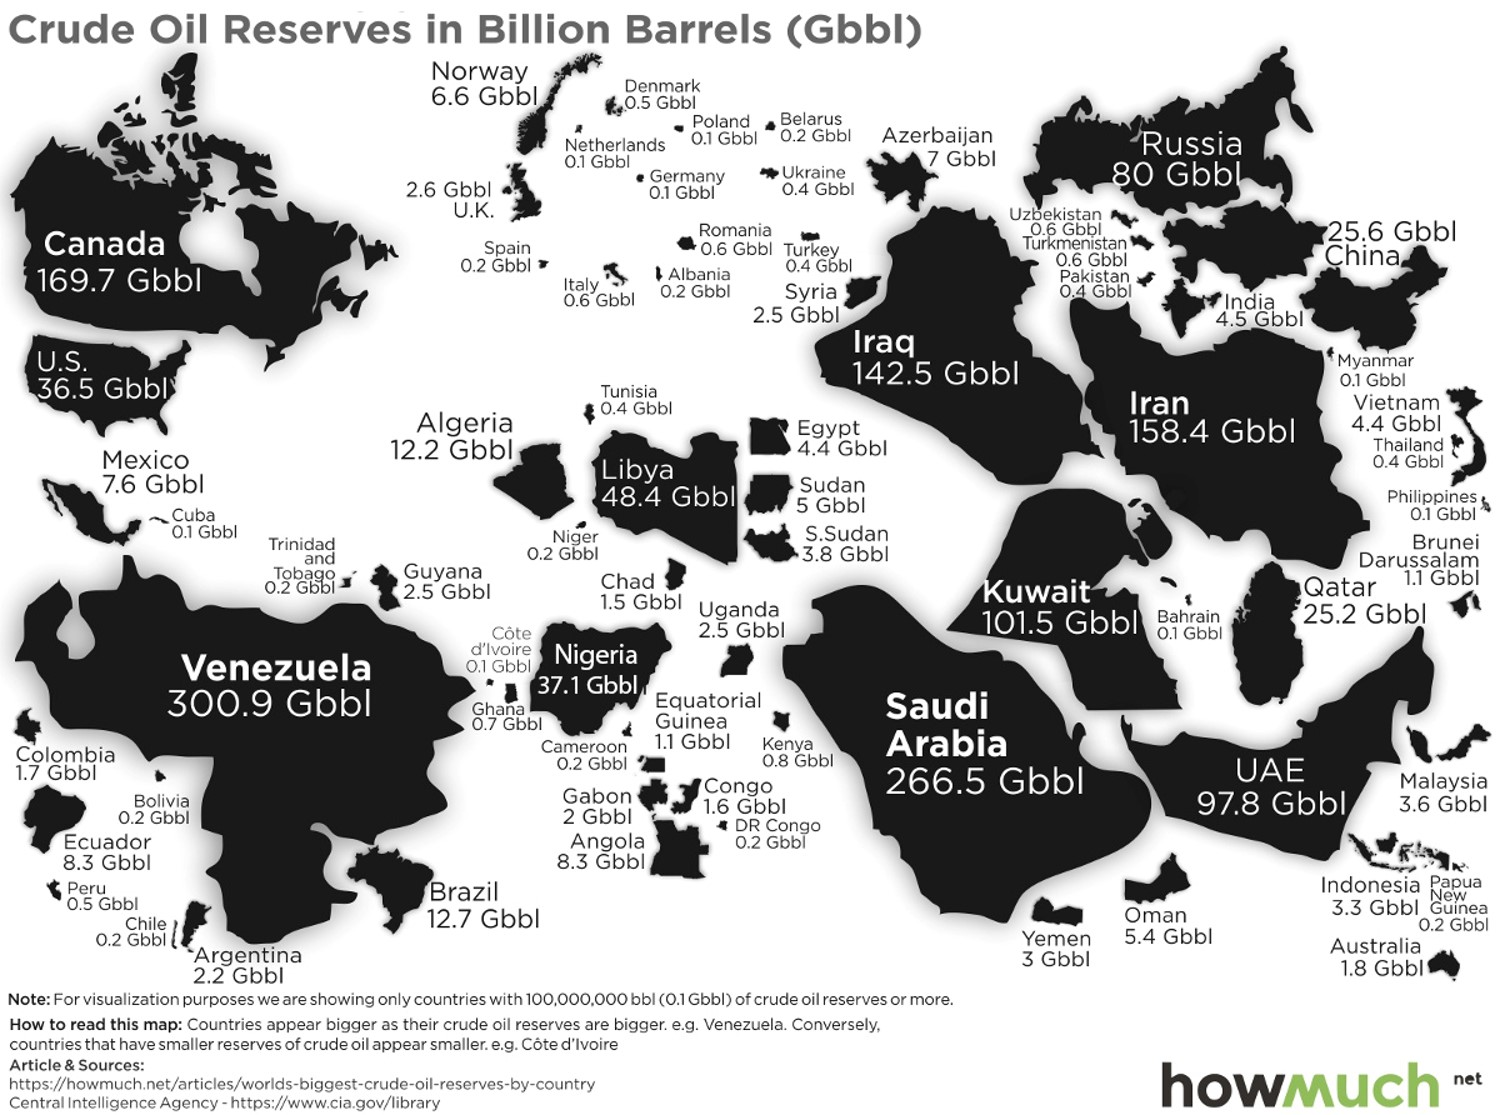
\includegraphics[width=\textwidth,height=0.9\textheight,keepaspectratio]{oil distribution.jpg}
\end{frame}


% Input from Navin's chapter
\begin{frame} 
	\frametitle{\LARGE{The Petrodollar System}}
	\begin{itemize}
		
		\item Oil is also special because the USD is tied to oil. \pause 
		\item Bapat (2019) compares the \textbf{petrodollar system} to the gold standard and Bretton Woods. \pause 
		\begin{itemize}
			\item US convinces Saudi Arabia to sell oil exclusively in USD... \pause 
			\item ...in exchange for respecting regime and territory (e.g. First Gulf War) \pause 
			\item Saudi Arabia re-invests those USD in US bonds.  \pause 
			\item Ensures USD is the most widely-used reserve currency while enabling the US government to easily fund itself.   
		\end{itemize}
		
	\end{itemize}
\end{frame}


\begin{frame} 
	\frametitle{\LARGE{The Petrodollar System}}
	\begin{itemize}
		
		\item Bapat argues 9/11 gave US pretext to invade Iraq to prevent destabilization of petrodollar system, as Saddam was threatening to sell in Euros.  \pause 
		\begin{itemize}
			\item Also informs US interpretation of Iran and Venezuela as existential threats despite the military power disparity.  \pause 
			\item US projects force globally to protect major oil-transport waterways. \pause 
		\end{itemize}
		\item Any instability in a major oil producer becomes threatening to this system, so US may contribute to autocratic stability when trying to keep this system stable.
		
	\end{itemize}
\end{frame}


% Saudi ARabia debt
%\begin{frame}{\LARGE Impending Fiscal Crisis in Saudi Arabia?}
%    \centering
%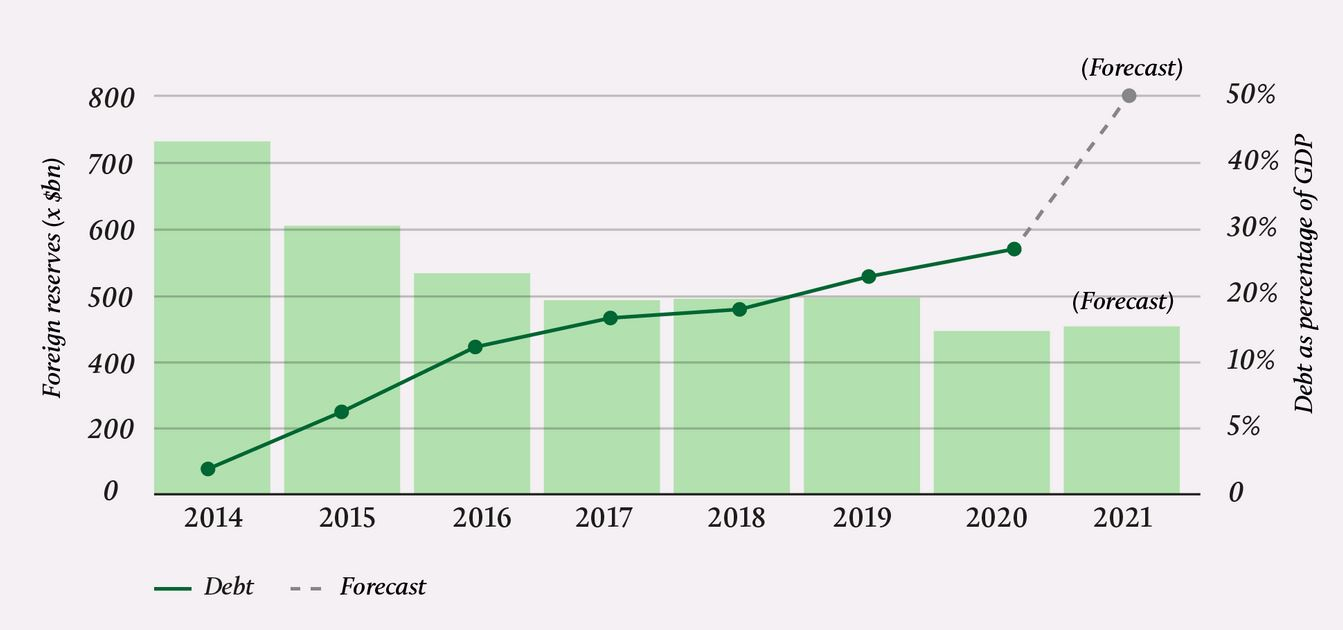
\includegraphics[width=\textwidth,height=0.8\textheight,keepaspectratio]{saudi arabia debt.JPG}
%\end{frame}

\begin{frame} 
	\frametitle{\LARGE{Endogeneity and the Resource Curse}}
	\begin{itemize}
		\large{
			\item Recall the concept of endogeneity: the resource curse may be observed because we are missing some other important factor.
			\item Endogeneity can be due to common cause, reverse causation, or spurious association.
			\begin{itemize}
				\item Weak political institutions or poor economic growth are not random. \pause 
				\item Institutions and the economy may be the \textbf{cause} of the curse, not the result. \pause 
			\end{itemize}
			\item Ross (2015) emphasizes a number of studies which attempt to grapple with this problem.   
			
		}
	\end{itemize}
\end{frame}

%% Slide outline
\begin{frame} 
	\frametitle{\LARGE{Is the Curse Real?}}
	\begin{itemize}
		\large{ 
			\item Economically: strong theories and associations for the resource curse. \pause
			
			\item Politically: \pause
			\begin{itemize}
				\item Civil conflict association is real, but no theory to explain. \pause
				\item May be conditional upon pre-existing domestic institutions: \pause
				\begin{itemize}
					\item Makes autocracies more autocratic and less accountable. \pause
					\item Less clear effect on democracies, but may undermine weak democracies. \pause
				\end{itemize}
				
			\end{itemize}
			\item Oil appears to be a special case, due to its unique characteristics: \pause
			\begin{itemize}
				\item The major input into world production and trade\pause
				\item US influence through petrodollar system 
			\end{itemize}
		}
	\end{itemize}
\end{frame}

\begin{frame} 
	\frametitle{\LARGE{Solutions}}
	\begin{itemize}
		\large{
			\item Best case: have transparent, accountable, domestic political institutions in place to manage resource extraction before it starts. \pause
			\begin{itemize}
				\item Botswana has \href{https://openknowledge.worldbank.org/handle/10986/18304}{successfully managed} its resource wealth\pause
			\end{itemize}
			
			\item Have an already-diversified economy when resources are discovered. \pause
			\begin{itemize}
				\item Abundance is not the problem; \textit{dependence is} \pause
				\item Canada vs. Democratic Republic of Congo\pause
			\end{itemize}
			
			\item Attaining either one of these features \textit{after} discovering resources is incredibly difficult. \pause
			\begin{itemize}
				\item This is the resource curse in a nutshell: the best solutions are undermined by the very existence of the problem. 
			\end{itemize}
		}
	\end{itemize}
\end{frame}






\end{document}
